\documentclass[twoside]{scrartcl}

%\usepackage[blacklinks]{drangreport}
\usepackage[bluelinks]{drangreport}

%\usepackage{cmbright}

\usepackage{pgfplots}

%Thomas' contradiction symbol
\newcommand*{\cont}{%
  \mathsf{X}\mkern-8.5mu\mathsf{X}%
}
\renewcommand{\thempfootnote}{$\dagger$}

%Change font of proof to scshape, not sure if it looks better...
%\expandafter\let\expandafter\oldproof\csname\string\proof\endcsname
%\let\oldendproof\endproof
%\renewenvironment{proof}[1][\proofname]{%
%  \oldproof[\scshape #1]%
%}{\oldendproof}


\title{Analysis I}


\hypersetup{pdfinfo={
Title={Analysis I Lecture Notes},
Author={Karim Bacchus},
Keywords ={Analysis I, M1P1, Lecture Notes, Imperial College, Maths},
}}


\begin{document}


\NotesTitle{1st}{Spring 2015}{Analysis I}{Prof. R. P. W.}{Thomas}
{

\section*{Syllabus}  

\textit{A rigorous treatment of the concept of a limit, as applied to sequences, series and functions.}

\subsubsektion{Sequences}\vspace*{-5pt}
Real and complex sequences. Convergence, divergence and divergence to infinity. Sums and products of convergent sequences. The Sandwich Test. Sub-sequences, monotonic sequences, Bolzano-Weierstrass Theorem. Cauchy sequences and the general principle of convergence.

\subsubsektion{Series}\vspace*{-5pt}
Real and complex series. Convergent and absolutely convergent series. The Comparison Test for non-negative series and for absolutely convergent series. The Alternating Series Test.  Rearranging absolutely convergent series. Radius of convergence of power series. The exponential series.

\subsubsektion{Continuity}\vspace*{-5pt}
Limits and continuity of real and complex functions. Left and right limits and continuity. Maxima
and minima of real valued continuous functions on a closed interval. Inverse Function Theorem for
strictly monotonic real functions on an interval. 

\subsubsektion{Differentiation}\vspace*{-5pt}
 An introduction to differentiability: definitions, examples, left and right derivative.

\subsection*{Appropriate books}

{\shortskip

K.~G.~ Binmore, \textit{Mathematical Analysis, A Straightforward Approach} (Cambridge University Press).

}

}

\TableofContents
%!TEX root = M1P1.tex

\stepcounter{lecture}
\pagebreak
\setcounter{section}{-1}

\setcounter{lecture}{-1}

\setcounter{page}{4}
\sektion{Preliminaries}

M1F stuff:\lecturemarker{1}{5 Oct}


\begin{itemize}
\item $\forall$ - for any, \textbf{fix any}, for all, every...
\item $\exists$ - there exists
\item $\N - \{1,2,3,\dots\}$ 
\end{itemize}

\begin{theorem}[Triangle Inequality]
(See Question Sheet 1)
	\[|a+b| \leq |a| + |b|\]
\end{theorem}

\begin{corollary}
\[\left||a| - |b|\right|\leq |a-b|	\]
\end{corollary}
\begin{proof}
\[
\begin{aligned}
|a-b| < \epsilon &\iff b-\epsilon < a < b + \epsilon\\
&\iff a \in (b-\epsilon, b+\epsilon)\\
&\iff b \in (a-\epsilon, a+\epsilon)	\\
&\implies \left||a| - |b|\right|< \epsilon
\end{aligned} \] 
\end{proof}

Lots of other versions, see Question Sheet 1 - \emph{don't try to memorise them!}\\



\begin{clicker}
Fix $a \iR$. What does the statement 
\[\forall \epsilon >0,~|x-a|<\epsilon \tag{$*$}\]
mean for the number $x$? 

\textbf{Answer:} $x = a$. 
\begin{proof}
Assume $x \neq a$. Take $\epsilon := \frac{1}{2}|x-a| > 0$. Then $(*)$ does not hold.	
\end{proof}

\end{clicker}




\sektion{Sequences}
\label{sub:sequences}

A \lecturemarker{2}{5 Oct}
sequence $(a_n)_{n\geq 1}$ of real (or complex, etc.) numbers is an infinite list of numbers $a_1,~a_2,~a_3,\dots$ all in $\mathbb{R}$ (or $\mathbb{C}$, etc.) Formally:\\

\begin{definition}
	A \emph{sequence} is a function $a:\mathbb{N} \to \mathbb{R}$
\end{definition}

\textbf{Notation:} We let $a_n \in \mathbb{R}$ denote $a(n)$ for $n \in \mathbb{N}$. The data $(a_n)_{n=1,2,\dots}$ is equivalent to the function $a:\mathbb{N} \to \mathbb{R}$ because a function $a$ is determined by its values $a_n$ over all $n \in \mathbb{N}$. 

We will denote $a$ by $a_1,~a_2,\dots$ or $(a_n)_{n\in\mathbb{N}}$ or $(a_n)_{n\geq 1}$ or even just $(a_n)$.\vspace*{5pt}

\begin{remark}
$a_i$'s could be repeated, so $(a_n)$ is \emph{not} equivalent to the set $\{a_n : n \in \mathbb{N}\}\subset \mathbb{R}$. E.g. $(a_n) = 1,~0,~1,~0,\dots$ is different from $(b_n) = 1,~0,~0,~1,~0,~0,~1,\dots$	
\end{remark}

We can describe a sequence in may ways, e.g. formula for $a_n$ as above $a_n = \frac{1-(-1)^n}{2}$, or a recursion e.g. $c_1 = 1 = c_2$, $c_n = c_{n-1} + c_{n-2}$ for $n\geq 3$, or a summation (see next section) e.g. $d_n = \sum_{i=1}^n \frac{1}{i} = 1 + \frac{1}{2} + \frac{1}{3} + \dots +\frac{1}{n}$.

\subsektion{Convergence of Sequences}
We want to \emph{rigorously} define $a_n \to a \in \mathbb{R}$, or ``$a_n$ converges to $a$ as $n \to \infty$" or ``$a$ is the limit of $(a_n)$". 

Idea: $a_n$ should get closer and closer to $a$. Not necessarily monotonically, e.g.:
\[a_n = 
\begin{cases}
\frac{1}{n} & n \text{ odd}\\
\frac{1}{2n} & n \text{ even}	
\end{cases}
\hspace*{20pt}\text{ we want } a_n \to 0\]


\begin{center}
\begin{tikzpicture}
\begin{axis}[axis lines=middle,
     x label style={at={(axis description cs:0.95,-0.15)}},
     y label style={at={(axis description cs:-0.1,0.9)}},
    xlabel={$n$},
    ylabel={$a_n$},
    ticks=none,
  ymin = 0,
  ymax = 0.4,
  xmin = 1,
  xmax = 10,
  width=10cm,height=5cm]
   \addplot[samples at={3,5,7,9}, only marks, mark=x, mark size=3pt]{1/x};
    \addplot[samples at={2,4,6,8},only marks,mark=x,mark size=3pt]{(1/(2*x))};
  \end{axis}
\end{tikzpicture}
\end{center}
Also notice that $\frac{1}{n}$ gets closer and closer to $-1$! So we want to say instead that $a_n$ gets \emph{as close as we like to $a$}. We will measure this with $\epsilon >0$. We phrase ``$a_n$ gets \emph{arbitrarily} close to $a$" by ``$a_n$ gets to within $\epsilon$ of $a$ for \emph{any} $\epsilon >0$".\\

\begin{definition}[Mestel]
	$u_n \to u$ if $\forall n$ sufficiently large, $|u_n - u|$ is \emph{arbitrarily small.} 
	
Define a real number $b \in \mathbb{R}$ to be arbitrarily small if it is smaller than any $\epsilon >0$ i.e. $\forall \epsilon >0,~|b| < \epsilon$.
\end{definition}

Definition Mestel says that once $n$ is large enough, $|u_n - u|$ is less than every $\epsilon >0$, i..e it's zero, i.e. $u_n = u$. We want to \emph{reverse} the order of specifying $n$ and $\epsilon$. 

i.e. we want to say that to get \emph{arbitrarily close to the limit $a$} (i.e. $|a_n - a| < \epsilon$), we need to go sufficiently far down the sequence. Then if I change $\epsilon >0$ to be smaller, I simply go further down the sequence to get within $\epsilon$ of $a$. 

\begin{center}
\begin{tikzpicture}
\begin{axis}[
 axis line style={red},
axis lines=middle,
     x label style={at={(axis description cs:1.05,0.33)}},
     y label style={at={(axis description cs:-0.1,1.1)}},
    xlabel={\small $n$},
    ylabel={$a_n \to 0$},
  ymin = -0.4,
  ymax = 0.7,
  xmin = 1,
  xmax = 20,
    ytick = {0.3,0.12},
   yticklabels={$\epsilon_1$,$\epsilon_2$},
   xtick = 0,
  width=12cm,height=8cm]
   \addplot[samples at={2,...,20}, only marks, mark=x, mark size=2pt,  mark options={red},]{1/x};
   \draw (axis cs:20,0.3) -- (axis cs:0,0.3);
      \draw (axis cs:20,0.12) -- (axis cs:0,0.12);
     \draw (axis cs:20,-.1) -- (axis cs:4,-.1) node at (axis cs:10,-0.15){\small $n$ suff. large for $|a_n - 0| < \epsilon_1$};
          \draw (axis cs:4,-.06) -- (axis cs:4,-.1);
          \draw (axis cs:20,-.06) -- (axis cs:20,-.1);
          \draw (axis cs:20,-.25) -- (axis cs:9,-.25) node at (axis cs:15,-0.3){\small $n$ suff. large for $|a_n - 0| < \epsilon_2$};
           \draw (axis cs:9,-.2) -- (axis cs:9,-.25);
          \draw (axis cs:20,-.2) -- (axis cs:20,-.25);

  \end{axis}
\end{tikzpicture}
\end{center}

There will not be a ``$n$ sufficiently large" that works for all $\epsilon$ at once! (unless $a_n = a$ eventually.)

But for \emph{any} (fixed) $\epsilon>0$ we want there to be an $n$ sufficiently large such that $|a_n - a| < \epsilon$. So we change ``$\exists n$ such that $\forall \epsilon$" to ``$\forall \epsilon,~\exists n.$". \emph{This allows $n$ to depend on $\epsilon$.}~\\

\begin{definition}[Nestel]
	$a_n \to a$ if $\forall \epsilon >0,~\exists n \in \mathbb{N}$ such that $|a_n - a| < \epsilon$. 
\end{definition}

e.g. 
\[
a_n = \begin{cases}
 0 & n\text{ even}\\
 1 & n\text{ odd}	
 \end{cases}
 \text{ satisfies } a_n \to 0 \text{ according to Prof. Nestel.}
\]

We want to modify this to say eventually $|a_n - a| < \epsilon$ \emph{and it stays there!}\vspace*{5pt}

\textbf{Ignore Mestel and Nestel's definition!}\lecturemarker{3}{5 Oct}\\

\begin{definition}[Convergence]
We say that $a_n \to a$ iff 
\[\forall \epsilon >0,~\exists N \in \mathbb{N} \text{ such that } ``n \geq N \implies |a_n - a| < \epsilon"\]	
\end{definition}

This says that \emph{however close} ($\forall \epsilon>0$) I want to get to the limit $a$, there's a point in the sequence ($\exists N \in \mathbb{N}$) beyond which ($n \geq N$) my $a_n$ is indeed that close to the limit $a$ ($|a_n - a| <\epsilon$).\\ 

\begin{remark}
$N$ depends on $\epsilon$! $N = N(\epsilon)$	
\end{remark}

Equivalently:
\[\forall \epsilon >0,~ \exists N \in \mathbb{N} \text{ such that} ``\forall n \geq N,~|a_n -a|<\epsilon"\]
or equivalently
\[\forall \epsilon >0,~\exists N_\epsilon\in\mathbb{N} \text{ such that } |a_n - a| < \epsilon,~\forall n \geq N_\epsilon\]

\begin{clicker}Given a sequence of real numbers $(a_n)_{n\geq 1}$. Conisder 
\[\boxed{\forall n \geq 1,~\exists \epsilon >0 \text{ such that } |a_n|< \epsilon}\]
This means? 

\textbf{Answer:} It always holds. \begin{proof}
 Fix any $n \in \mathbb{N}$. Take $\epsilon = |a_n| + 1$. 	
 \end{proof}
 
What about
 \[\boxed{\exists \epsilon >0 \text{ such that } \forall n \geq 1,~|a_n| < \epsilon} \]
 
 \textbf{Answer:} $(a_n)$ is bounded.
 
 
\begin{center}
\begin{tikzpicture}
\begin{axis}[
 axis line style={red},
axis lines=middle,
     x label style={at={(axis description cs:1.05,0.4)}},
     y label style={at={(axis description cs:-0.1,1.1)}},
    xlabel={\small $n$},
    ylabel={$a_n$},
  ymin = -0.4,
  ymax = 0.4,
  xmin = 1,
  xmax = 10,
     ytick = {0.3, -.3},
   yticklabels={$\epsilon$,$-\epsilon$},
   xtick = 0,
  width=10cm,height=5cm]
   \addplot[samples at={5,7,9}, only marks, mark=x,  mark options={red}, mark size=3pt]{(-1)^x*1/x};
    \addplot[samples at={2,3,4,6,8},only marks, mark options={red},mark=x,mark size=3pt]{(1/(2*x))};
       \draw (axis cs:20,0.3) -- (axis cs:0,0.3);
      \draw (axis cs:20,-0.3) -- (axis cs:0,-0.3);
  \end{axis}
\end{tikzpicture}
\end{center}


  \begin{proof}
$\iff a_n \in (-\epsilon,\epsilon)~ \forall n \iff |a_n|$ is bounded by $\epsilon$. \end{proof}

\end{clicker}~

\begin{definition}
If $a_n$ does not converge to $a$ for any $a\in \mathbb{R}$, we say that $a_n$ \emph{diverges.}
\end{definition}~

\begin{example}
I claim that $\frac{1}{n} \to 0$ as $n \to \infty$

\textit{Rough working:} Fix $\epsilon >0$. I want to find $N \in \mathbb{N}$ such that $|a_n - a| = |\frac{1}{n} - 0| = \frac{1}{n} < \epsilon$ for all $n \geq N$. 
\begin{center}
\begin{tikzpicture}
\begin{axis}[
 axis line style={red},
axis lines=middle,
     x label style={at={(axis description cs:1.05,0.1)}},
     y label style={at={(axis description cs:-0.1,1.1)}},
    xlabel={\small $n$},
    ylabel={$a_n$},
  ymin = -0.1,
  ymax = 0.4,
  xmin = 1,
  xmax = 10,
     ytick = {0.15},
   yticklabels={$\epsilon$},
   xtick = 0,
  width=10cm,height=5cm]
   \addplot[samples at={5,7,9}, only marks, mark=x,  mark options={red}, mark size=3pt]{(-1)^x*1/x};
    \addplot[samples at={2,3,4,6,8},only marks, mark options={red},mark=x,mark size=3pt]{(1/(2*x))};
       \draw (axis cs:20,0.15) -- (axis cs:0,0.15);
        \draw (axis cs:4,0.12) -- (axis cs:4,-0.1) node at (axis cs:4.2,-0.05) {$N$};
  \end{axis}
\end{tikzpicture}
\end{center}


Since $a_n = \frac{1}{n}$ is monotonic, it is \emph{sufficient} to ensure that $\frac{1}{N} < \epsilon \iff N > \frac{1}{\epsilon}$ (This \emph{implies} $\frac{1}{n} \leq \frac{1}{N} < \epsilon,~\forall n \geq N$).

\begin{proof}
Fix $\epsilon >0$. 
 Pick any $N \in \mathbb{N}$ such that $N > \frac{1}{\epsilon}$. (This is the Archimedean axiom of $\mathbb{R}$. Notice $N$ depends on $\epsilon$!!). Then $n \geq N \implies |\frac{1}{n}-0| = \frac{1}{n} \leq \frac{1}{N} < \epsilon$.
\end{proof}


\end{example}


\textbf{Method to prove $a_n \to a$}
\begin{enumerate}
\item[(I)] Fix $\epsilon > 0$
\item[(II)] Calculate $|a_n - a|$
\item[(II$'$)] Find a good estimate $|a_n - a| < b_n$
\item[(III)] Try to solve $a_n - a < b_n < \epsilon ~~(*)$
\item[(IV)] Find $N \in \mathbb{N}$ s.t. $(*)$ holds whenever $n \geq N$
\item[(V)] Put everything together into a logical proof (usually involves rewriting everything in reverse order - see examples below)
\end{enumerate}~

\begin{example}
$a_n = \dfrac{n+5}{n+1}$\\

\emph{Rough Working}
\[ |a_n - 1| = \left| \dfrac{n+5}{n+1} -1 \right| = \dfrac{4}{n+1}\]

This is $< \epsilon \iff n+1 > 4/\epsilon \iff n > 4/\epsilon$, so take $N \geq 4/\epsilon$. 

\begin{proof}
Fix $\epsilon > 0$. Pick $N$ such that $N \geq 4/\epsilon$. Then $\forall n \geq N$, \[|a_n - 1| = \frac{4}{n+1} \leq \frac{4}{N+1} < \frac{4}{N} \leq \epsilon\qedhere\]
\end{proof}
\end{example}~

\begin{example}$a_n = \dfrac{n+2}{n-2} \to 1$\\

\emph{Rough Working} 
\[|a_n -1| = \left|\frac{n+2}{n-2} - 1\right| = \frac{4}{n-2}\]

We want $\frac{4}{n-2} < \epsilon$. We want implications in the $\impliedby$ direction (i.e. $\frac{4}{n-2} < \epsilon \impliedby n \geq N$) \emph{not} $\implies$ direction. i.e. $\frac{4}{n-2} < \epsilon \implies \frac{4}{n} < \epsilon$.

But if we take $N = \frac{4}{\epsilon}$, we need the \emph{opposite} implication, we \emph{need} $\frac{4}{n-2} < \epsilon$. We \emph{need} to estimate $\frac{4}{n-2} < b_n$, and then solve $b_n < \epsilon$. So we make denominator smaller. 

To make $n-2$ smaller, make $2$ bigger! e.g. $\frac{n}{2}>2$ for $n>4$. Then $\frac{4}{n-2} < \frac{4}{n-n/2} = \frac{8}{n}$

Also want $b_n = \frac{8}{n} < \epsilon \iff n > 8/\epsilon$. So take $N > \mathrm{max}(8/\epsilon, 4)$.

\begin{proof}
Fix $\epsilon > 0.$	Choose $N \iN$ such that $N > \mathrm{max}(8/\epsilon, 4)$. Then $n \geq N \implies n > 8/\epsilon~ (1)$ and $n > 4 ~(2) \implies$

\[\left|\frac{n+2}{n-2} - 1\right| = \frac{4}{n-2} \underbrace{<}_{(2)} \frac{4}{n-n/2} = \frac{8}{n} \underbrace{<}_{(1)} \epsilon\qedhere\]

\end{proof}

	
\end{example}
\pagebreak


\lecturemarker{4}{5 Oct}
We can also define limits for \emph{complex sequences}.\\

\begin{definition}
$a_n \in \mathbb{C},~\forall n \geq 1$. We say $a_n \to a \in \mathbb{C}$ iff
\[\forall \epsilon >0,~\exists N \in \mathbb{N} \text{ such that } n \geq N \implies |a_n - a| < \epsilon\]	

(i.e. $\sqrt{\Re(a_n-a)^2 + \frak{I}(a_n-a)^2} < \epsilon$) 

This is equivalent (see problem sheet!) to $(\frak{R}a_n) \to \frak{a}$ \emph{and} $(\frak{I}a_n) \to \frak{I}a$
\end{definition}~

\begin{example}
Prove $a_n = \dfrac{e^{in}}{n^3-n^2-6} \to 0$ as $n \to \infty$\\

\emph{Rough Working} 
\[|a_n - a| = \left|\dfrac{e^{in}}{n^3-n^2-6} \right| = \left|\frac{1}{n^3-n^2-6}\right|\]

\emph{Estimate} $\left|\dfrac{1}{n^3-n^2-6}\right| < \dfrac{1}{c_n}$ by making $c_n$ smaller than $n^3 - n^2 - 6$ (But not too small! We want $c_n \to \infty$). So let $c_n = n^3 - \text{\emph{ something bigger than} } n^2 + 6$.

Take off $\frac{n^3}{2}$ to make the expression simple. For $n \geq 4$, we have $\frac{n^3}{2} > n^2 + 6$. 

So for $n \geq 4$
\[\left|\frac{1}{n^3-n^2-6}\right| < \frac{1}{n^3- n^3/2} = \frac{2}{n^3} \]
and this is $< \epsilon$ for $n > \sqrt[3]{\frac{2}{\epsilon}}$.

\begin{proof}
$\forall \epsilon > 0$, choose $N \geq \mathrm{max}(4,\sqrt[3]{2/\epsilon})$	. Then $\forall n \geq N$
\[|a_n - 0| = \left| \frac{1}{n^3-n^2 - 6}\right| < \frac{1}{n^3- n^3/2} = \frac{2}{n^3} \leq \frac{2}{N^3} \leq \epsilon \qedhere \]
\end{proof}
\end{example}~


\begin{example}
Set $\delta = 10^{-1000000}, ~a_n = (-1)^n\cdot\delta$. Prove that $a_n$ does not converge. 

We want to show that the following is false: 
\[\exists a \text{ s.t. } \forall \epsilon > 0,~\exists N \in \mathbb{N} \text{ s.t. } n \geq N \implies |a_n - a| <\epsilon\]
i.e. we need to prove
\[\forall a,~ \exists \epsilon > 0 \text{ s.t. } \forall N \in \mathbb{N},~\exists n \geq N \text{ s.t. } |a_n-a| \geq \epsilon\]

\emph{Rough:} 	
Assume for contadiction that $a_n \to a$, i.e. $\forall \epsilon > 0,~\exists N \in \mathbb{N} \text{ s.t. } n \geq N \implies |a_n - a| <\epsilon$


\begin{center}
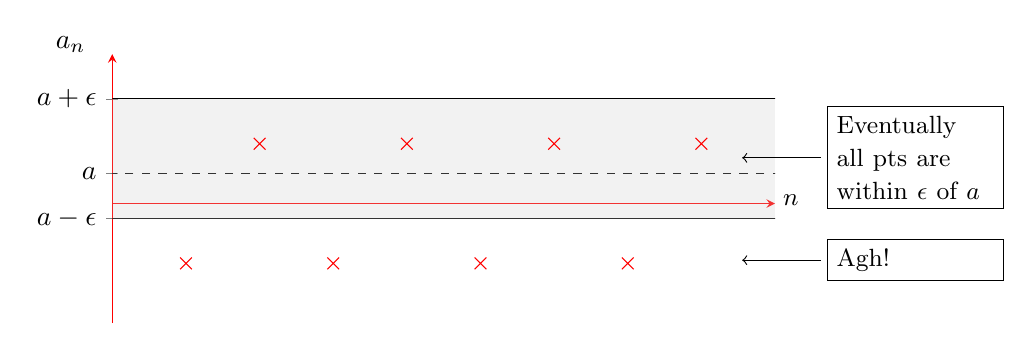
\begin{tikzpicture}
\begin{axis}[
 axis line style={red},
axis lines=middle,
     x label style={at={(axis description cs:1.05,0.4)}},
     y label style={at={(axis description cs:-0.1,1.1)}},
    xlabel={\small $n$},
    ylabel={$a_n$},
  ymin = -0.4,
  ymax = 0.5,
  xmin = 1,
  xmax = 10,
     ytick = {0.35, -0.05,0.1},
   yticklabels={$a+\epsilon$,$a-\epsilon$, $a$},
   xtick = 0,
  width=10cm,height=5cm]
   \addplot[samples at={3,5,7,9}, only marks, mark=x,  mark options={red}, mark size=3pt]{0.2};
    \addplot[samples at={2,4,6,8,},only marks, mark options={red},mark=x,mark size=3pt]{-0.2};
       \draw (axis cs:20,0.35) -- (axis cs:0,0.35); %a+e line
      \draw (axis cs:20,-0.05) -- (axis cs:0,-0.05); %a-e line
       \draw[dashed] (axis cs:20,0.1) -- (axis cs:0,0.1); %a line
         \fill[gray!40,nearly transparent] (axis cs:0,-.05)-- (axis cs: 0,0.35) -- (axis cs: 10,0.35) -- (axis cs: 10,-0.05) -- cycle;
  \end{axis}
   \draw[->] (9,2.1) -- (8,2.1);
      \draw[->] (9,0.8) -- (8,0.8);
      \node[draw,text width=2cm] at (10.2,2.1) {\small Eventually all pts are within $\epsilon$ of $a$};
        \node[draw,text width=2cm] at (10.2,0.8) {\small Agh!};
\end{tikzpicture}
\end{center}


For small enough $\epsilon >0$, the fact that $a$ is within $\epsilon$ of $\delta ~ (a_{2n})$ and $-\delta ~(a_{2n+1})$ will be a contradiction. 


\begin{proof}
Fix $a\iR$. Take $\epsilon = \delta$ (or $\epsilon < \delta$ will do). 

 Then if $\exists N$ s.t. $\forall n \geq N$, $|a_n - a| <\epsilon$ this implies
\begin{enumerate}
\item $|a_{2N} - a | < \epsilon \iff a \in (\delta - \epsilon, \delta + \epsilon)\implies a > \delta - \epsilon =0$ 
\item $|a_{2N+1} - a | < \epsilon\iff a \in (-\delta - \epsilon,-\delta + \epsilon) \implies a < -\delta + \epsilon = 0,~\cont$ 
\end{enumerate}
(or use triangle inequality: \[|\delta - (-\delta)| \leq |\delta - a| + |a -(-\delta)| < \epsilon + \epsilon \implies 2\delta < 2\epsilon = 2\delta ~\cont\text{)}\]
So $a_n \not\to a$, but this holds $\forall a \in \RR$, so $a_n$ does not converge.
\end{proof}
\end{example}~

\begin{clicker}
Fix $(a_n)_{n\geq 1},~a_n \in \RR$. Then \[\forall n,~\exists \epsilon >0 \text{ s.t. } |a_n| < \epsilon \text{ means?}\]

\textbf{Answer:} Nothing. This is always true. Take $\epsilon = |a_n| + 1$	
\end{clicker}~

\lecturemarker{5}{5 Oct}

\begin{theorem}[Uniqueness of Limits]
Limits are unique. If $a_n \to a$ and $a_n \to b$, then $a=b$	
\end{theorem}

\emph{Idea:} For $n$ large, $a_n$ should be close to $a$ and to $b$. So $a$ arbitrarily close to $b \implies a = b$. 

\begin{proof}[Proof 1]~
\begin{enumerate}
\item $\forall \epsilon,~\exists N_a$ s.t. $\forall n \geq N_a,~|a_n - a| < \epsilon$ 

\item $\forall \epsilon,~\exists N_b$ s.t. $\forall n \geq N_b,~|a_n - b| < \epsilon$
\end{enumerate}

Set $N = \mathrm{max}(N_a,N_b)$. Then $\forall n \geq N$, (i) and (ii) hold, so
\[|a - b| = |(a-a_n) + (a_n - b)| \leq |a - a_n| + |a_n - b| < 2\epsilon \implies |a-b| = 0!\qedhere\]
(recall! if not, set $\epsilon = \frac{1}{2}|a-b| >0$ to get a contradiction)
\end{proof}~


\begin{proof}[Proof 2]
By contradiction. Assume $a \neq b$. 

\begin{center}
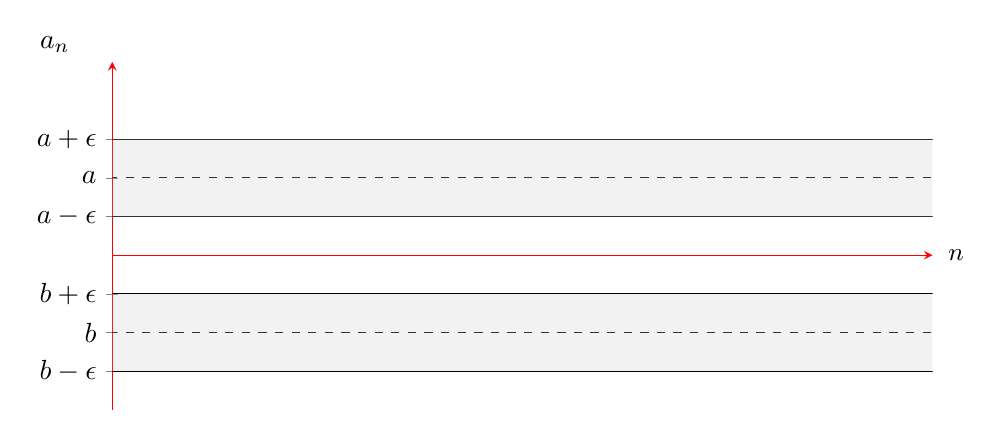
\begin{tikzpicture}
\begin{axis}[
 axis line style={red},
axis lines=middle,
     x label style={at={(axis description cs:1.05,0.4)}},
     y label style={at={(axis description cs:-0.1,1.1)}},
    xlabel={\small $n$},
    ylabel={$a_n$},
  ymin = -0.4,
  ymax = 0.5,
  xmin = 1,
  xmax = 10,
     ytick = {0.3, 0.2,0.1,-0.1,-0.2,-0.3},
   yticklabels={$a+\epsilon$,$a$, $a-\epsilon$,$b+\epsilon$, $b$, $b-\epsilon$},
   xtick = 0,
  width=12cm,height=6cm]
       \draw (axis cs:20,0.3) -- (axis cs:0,0.3); %a+e line
      \draw (axis cs:20,0.1) -- (axis cs:0,0.1); %a-e line
       \draw[dashed] (axis cs:20,0.2) -- (axis cs:0,0.2); %a line
         \fill[gray!40,nearly transparent] (axis cs:0,.1)-- (axis cs: 0,0.3) -- (axis cs: 10,0.3) -- (axis cs: 10,0.1) -- cycle;
         
          \draw(axis cs:20,-0.3) -- (axis cs:0,-0.3); %b+e line
      \draw (axis cs:20,-0.1) -- (axis cs:0,-0.1); %b-e line
       \draw[dashed]  (axis cs:20,-0.2) -- (axis cs:0,-0.2); %b line
         \fill[gray!40,nearly transparent] (axis cs:0,-.1)-- (axis cs: 0,-0.3) -- (axis cs: 10,-0.3) -- (axis cs: 10,-0.1) -- cycle;
  \end{axis}
\end{tikzpicture}
\end{center}

Eventually $a_n$ is in \emph{both} corridors. So if I choose $\epsilon$ sufficiently small so that corridors don't overlap to get a contradiction.

Set $\epsilon = \frac{|a-b|}{2} > 0$. Then $\exists N_a, N_b$ such that $\forall n \geq N_a,N_b$, we have 
\[|a_n - a| < \epsilon \text{ and } |a_n - b| < \epsilon\]
w.l.o.g. $a > b$. Then $a_n > a - \epsilon$ and $a_n < b$
\[\begin{aligned}
	&\implies b + \epsilon > a-\epsilon\\
	&\implies 2\epsilon > a-b = 2\epsilon~ \cont 
\end{aligned}\]
\end{proof}

\begin{clicker}
Prove $\frac{1}{n-2} \to 0$. Student Answer:
Fix $\epsilon >0$.
\begin{enumerate}
	\item We want $|\frac{1}{n-2} - 0| = \frac{1}{n-2} < \epsilon$
	\item $\implies n-2 > 1/\epsilon$
	\item $\implies n > 2 + 1/\epsilon$
	\item $\implies n > 1/\epsilon ~(*)$
	\item So take $N > 1/\epsilon$, then
	\item $\forall n \geq N$, $n > 1/\epsilon$ which is $(*)$
	\item So $\frac{1}{n-2} \to 0$
	\item (This is correct)
\end{enumerate}

\textbf{Answer:} (iv) is wrong. 
	
\end{clicker}


\begin{theorem}[Algebra of Limits]\label{thm1}
$a_n \to a$ and $b_n \to b$ then:\begin{enumerate}
\item $a_n+b_n \to a+b$
\item $a_nb_n \to ab$
\item $\frac{a_n}{b_n} \to \frac{a}{b} ~(b \neq 0)$
\end{enumerate}
\end{theorem}
\begin{proof}[Proof of (i)]
Fix any $\epsilon >0$. Then $\exists N_a \in \mathbb{N}$ such that $\forall n\geq N_a,~ |a_n	 - a| < \epsilon/2$ 

and $\exists N_b \in \mathbb{N}$ such that $\forall n \geq N_b,~ |b_n - b| < \epsilon/2$. Set $N =$ max$\{N_a,N_b\}$, so 
\[\begin{aligned}|(a_n + b_n) - (a+b)| &\leq |a_n -a| + |b_n -b| \\
	 &< \epsilon/2 + \epsilon/2 = \epsilon \qedhere
\end{aligned}\]
\end{proof}

\begin{proof}[Proof of (ii)]
\emph{Rough working:} 	
\[\begin{aligned}|a_nb_n -ab|  &= |(a_n -a)b - a_nb + a_nb_n|\\ 
&\leq |a_n-a||b| + |a_n|	|b_n-b|
\end{aligned}
\]

We can easily make $|a_n - a| < \epsilon/2$ if I take $|a_n - a| < \frac{\epsilon}{2|b|}$.

We need to show that $|a_n| < A$, so that I can take $|b_n - b| < \frac{\epsilon}{2A}$.\\

\begin{lemma}
If $a_n \to a$, then $(a_n)$ is bounded: $\exists A \in \RR \text{ s.t. }|a_n| < A,~\forall n$.
\end{lemma}
\begin{proof}[Proof of Lemma]~

\begin{center}
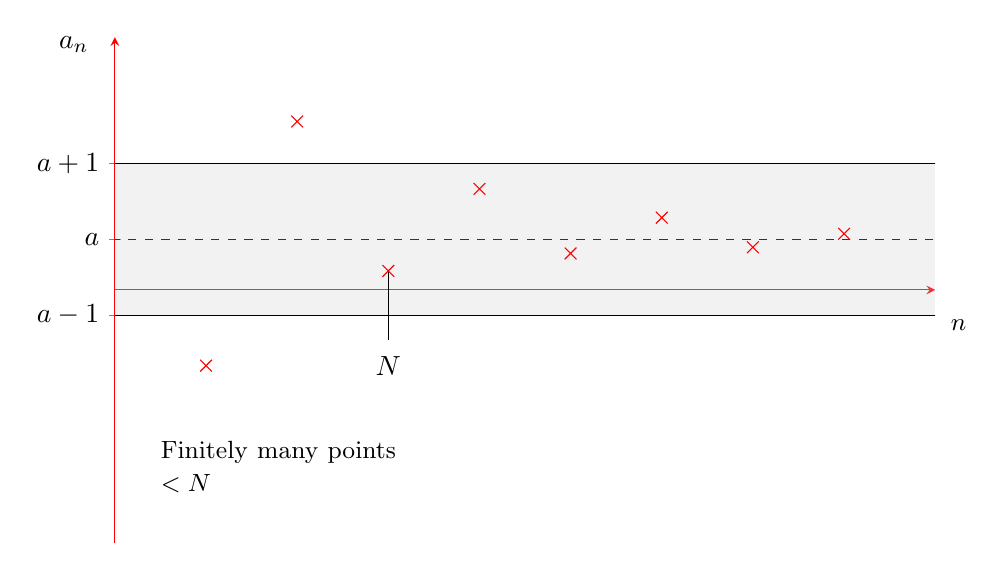
\begin{tikzpicture}
\begin{axis}[
 axis line style={red},
axis lines=middle,
     x label style={at={(axis description cs:1.05,0.4)}},
     y label style={at={(axis description cs:-0.08,1.02)}},
    xlabel={\small $n$},
    ylabel={$a_n$},
  ymin = -0.5,
  ymax = 0.5,
  xmin = 1,
  xmax = 10,
     ytick = {0.25, -0.05,0.1},
   yticklabels={$a+1$,$a-1$, $a$},
   xtick = 0,
  width=12cm,height=8cm]
   \addplot[samples at={3,5,7,9}, only marks, mark=x,  mark options={red}, mark size=3pt]{1/x};
    \addplot[samples at={2,4,6,8},only marks, mark options={red},mark=x,mark size=3pt]{-1/(x^2)+0.1};
       \draw (axis cs:20,0.25) -- (axis cs:0,0.25); %a+e line
      \draw (axis cs:20,-0.05) -- (axis cs:0,-0.05); %a-e line
       \draw[dashed] (axis cs:20,0.1) -- (axis cs:0,0.1); %a line
         \fill[gray!40,nearly transparent] (axis cs:0,-.05)-- (axis cs: 0,0.25) -- (axis cs: 10,0.25) -- (axis cs: 10,-0.05) -- cycle;
            \draw (axis cs:4,0.0375) -- (axis cs:4,-0.1) node at (axis cs:4,-0.15) {$N$};
                  \node[text width=3cm] at (axis cs:2.8,-0.35) {\small Finitely many points $<N$};
            
  \end{axis}
\end{tikzpicture}
\end{center}

Fix $\epsilon =1$. Then $\exists N \in \NN$ such that $\forall n \geq N,~|a_n - a| < 1 \implies |a_n| < 1 + |a|$. 

Then $(a_n)$ is bounded by max$\{a_1,a_2,\dots,a_{N-1},a+1\}$.
\end{proof}


Fix $\epsilon >0$. Then $\exists N_a$ such that $\forall n \geq N_a$, $|a_n - a| < \dfrac{\epsilon}{2(|b| + 1)}$ (we add $1$ in case $|b| = 0$)
and $\exists N_b$ such that $\forall n \geq N_b$, $|b_n - b| < \dfrac{\epsilon}{2A}$. 

Set $N = \text{max}(N_a,N_b)$. Then $\forall n \geq N$
\[\begin{aligned}|a_nb_n -ab| &\leq |a_n-a||b_n| + |b_n-b||a|\\ 
&< \frac{\epsilon}{2}\frac{|b|}{|b|+1} + A\frac{\epsilon}{2A}\\ 
& < \epsilon/2 + \epsilon/2 = \epsilon\qedhere	
\end{aligned}
\]
\end{proof}

See exercise sheet for proof of \ref{thm1}(iii).\\

\begin{theorem}
If $(a_n)$ is bounded above \emph{and} monotonically increasing then $a_n$ is \emph{convergent}.
\end{theorem}

\emph{Idea:} 
\begin{center}
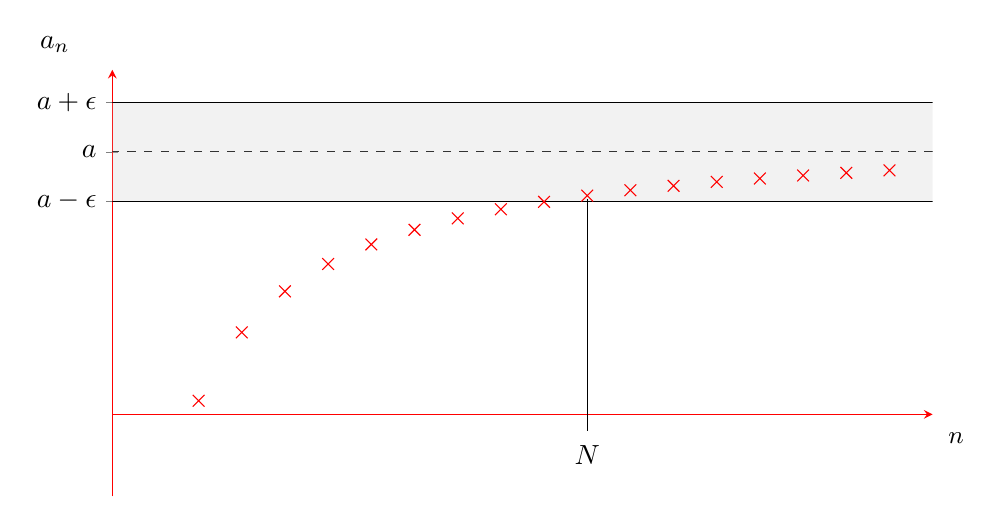
\begin{tikzpicture}
\begin{axis}[
 axis line style={red},
axis lines=middle,
     x label style={at={(axis description cs:1.05,0.1)}},
     y label style={at={(axis description cs:-0.1,1.1)}},
    xlabel={\small $n$},
    ylabel={$a_n$},
  ymin = -0.1,
  ymax = 0.42,
  xmin = 1,
  xmax = 20,
     ytick = {0.26,0.38,0.32},
   yticklabels={$a-\epsilon$,$a+\epsilon$,$a$},
   xtick = 0,
  width=12cm,height=7cm]
   \addplot[samples at={1,2,3,4,5,6,7,8,9,10,11,12,13,14,15,16,17,18,19}, only marks, mark=x,  mark options={red}, mark size=3pt]{0.35-1/x};
       \draw (axis cs:20,0.38) -- (axis cs:0,0.38);
              \draw (axis cs:20,0.26) -- (axis cs:0,0.26);
                     \draw[dashed] (axis cs:20,0.32) -- (axis cs:0,0.32);
         \fill[gray!40,nearly transparent] (axis cs:0,0.26)-- (axis cs: 0,0.38) -- (axis cs: 20,0.38) -- (axis cs: 20,0.26) -- cycle;
                     \draw (axis cs:12,0.262) -- (axis cs:12,-0.02) node at (axis cs:12,-0.05) {$N$};
  \end{axis}
\end{tikzpicture}
\end{center}
Eventually we get in the epsilon corridor (shaded area) because $a-\epsilon$ is \emph{not} an upper bound. We stay in there because monotonic and bounded by $a$.
\begin{proof}
Fix $\epsilon >0$. $a-\epsilon$ is \emph{not} an upper bound for $\{a_n : n \iN\}$ (because $a$ is the \emph{smallest} upper bound). So $\exists N \in \mathbb{N}$ such that $a_N > a-\epsilon$. Monotonic so $\forall n \geq N$ we have \[a\geq a_n\geq a_N > a-\epsilon \implies |a_n - a| < \epsilon\qedhere\]	
\end{proof}~

\begin{remark}\lecturemarker{6}{5 Oct}
 Now it's easier to handle things like $a_n = \dfrac{n^2 + 5}{n^3 - n + 6}$.

Dividing by $n^3$, we get $a_n = \dfrac{1/n + 5/n^3}{1 - 1/n^2 + 6/n^3}$.

 Use the fact that $1/n \to 0$ as $n \to \infty$ (Recall proof: $\forall \epsilon >0$, let $N_\epsilon  > 1/\epsilon$, then $n\geq N_{\epsilon} \implies n > 1/\epsilon \implies 1/n < \epsilon$), and the algebra of limits to deduce that 
\[a_n \to \dfrac{0 + 5.0^3}{1 - 0^2 + 6.0^3} = 0.\]
\end{remark}




\subsektion{Cauchy Sequences}
Gives a way of proving convergence \emph{without} knowing the limit.\\

\begin{definition}
	A sequence is Cauchy iff
	\[\forall \epsilon >0,~\exists N \in \mathbb{N} \text{ s.t. } \forall n,m \geq N,~ |a_n - a_m| < \epsilon\]
\end{definition}~

\begin{remark}
$m,n \geq N$ are arbitrary. It is not enough to say that $\forall \epsilon >0,~\exists N \in \NN$ such that $n \geq N \implies |a_n - a_{n+1}| < \epsilon$. See ex sheet. 	
\end{remark}

\begin{proposition}	
If $a_n \to a$ then $(a_n)$ is Cauchy. 
\end{proposition}
\begin{proof}
$a_n \to a\implies \forall \epsilon >0,~\exists N \text{ s.t. } n \geq N \implies |a_n - a| < \epsilon/2 ~(1)$


So $m \geq N \implies |a_m - a| < \epsilon /2 ~(2)$. So \[m,n \geq N \implies |a_n - a_m| \leq |a_n - a| + |a_m - a| < \underbrace{\epsilon/2}_{(1)} + \underbrace{\epsilon/2}_{(2)}=\epsilon\qedhere\]
\end{proof}

We want to prove converse: Cauchy $\implies$ Convergence.

We need a candidate for the limit $a$

\begin{center}
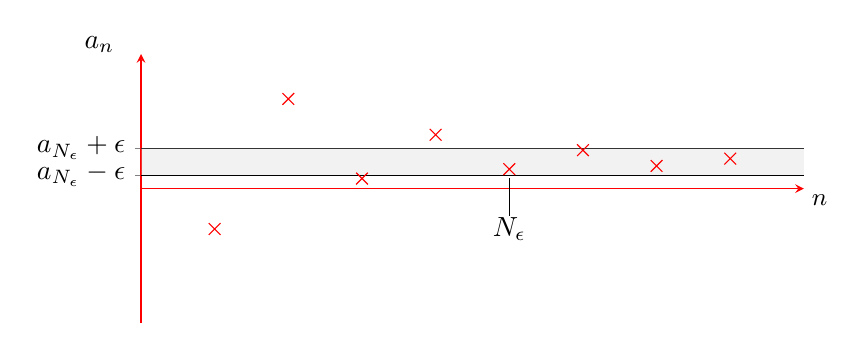
\begin{tikzpicture}
\begin{axis}[
 axis line style={red},
axis lines=middle,
     x label style={at={(axis description cs:1.05,0.4)}},
     y label style={at={(axis description cs:-0.1,1.1)}},
    xlabel={\small $n$},
    ylabel={$a_n$},
  ymin = -0.5,
  ymax = 0.5,
  xmin = 1,
  xmax = 10,
     ytick = {0.15, 0.05},
   yticklabels={$a_{N_{\epsilon}}+\epsilon$,$a_{N_{\epsilon}}-\epsilon$},
   xtick = 0,
  width=10cm,height=5cm]
   \addplot[samples at={3,5,7,9}, only marks, mark=x,  mark options={red}, mark size=3pt]{1/x};
    \addplot[samples at={2,4,6,8},only marks, mark options={red},mark=x,mark size=3pt]{-1/(x^2)+0.1};
       \draw (axis cs:20,0.15) -- (axis cs:0,0.15); %a+e line
      \draw (axis cs:20,0.05) -- (axis cs:0,0.05); %a-e line
       %\draw[dashed] (axis cs:20,0.1) -- (axis cs:0,0.1); %a line
         \fill[gray!40,nearly transparent] (axis cs:0,.05)-- (axis cs: 0,0.15) -- (axis cs: 10,0.15) -- (axis cs: 10,0.05) -- cycle;
            \draw (axis cs:6,0.04) -- (axis cs:6,-0.1) node at (axis cs:6,-0.15) {$N_\epsilon$};
     
            
  \end{axis}
\end{tikzpicture}
\end{center}

We will produce an auxiliary sequence which is \emph{monotonic} (+ bounded) $\implies$ convergence. $b_n:= \mathrm{sup}\{a_i : i \geq n\}$. Then picture shows that $b_{N_{\epsilon}} \in (a_{N_{\epsilon}} - \epsilon, a_{N_{\epsilon}} + \epsilon]$ and $b_n$'s are monotonically \emph{decreasing} because $b_{n+1} = \mathrm{sup}\{a_i : i \geq n+1\}$, a subset of $\{a_i : i \geq n\}$. 

So $b_n$s converge to $\mathrm{inf}\{b_n: n \iN\}$. We will show that $a_n$'s converge to same number, $a$, using Cauchy condition. 

\begin{lemma}
$(a_n)$ is Cauchy $\implies (a_n)$ is bounded
\end{lemma}

\begin{proof}
Pick $\epsilon =1$, then $\exists N$ such that $\forall n,m \geq N$, $|a_n - a_m|  < 1$. In particular $|a_n| < 1 + |a_N|~\forall n \geq N$ (take $m = N$), so 
\[|a_n| \leq \mathrm{max}\{|a_1|,|a_2|,\dots|a_{N-1}|,1+|a_N|\}~\forall N \iN\qedhere\]	
\end{proof}


\begin{theorem}
$(a_n)$ is a Cauchy sequence of real numbers $\implies a_n$ convergent. 
\end{theorem}

\begin{corollary}
$(a_n)$ Cauchy $\iff (a_n)$ convergent. (Ex: Show not true in $\QQ$!) 	
\end{corollary}

\begin{proof}
$(a_n)$ Cauchy $\implies$ bounded. So we can define $b_n = \mathrm{sup}\{a_i : i \geq n\}$. Then define $a = \mathrm{inf}\{b_n : n \iN\}$ and we prove that $a_n \to a$.

Fix $\epsilon > 0$. $\exists N \iN$ s.t. $n,m \geq N  \implies |a_n - a_m| < \epsilon/2 \iff a_n - \epsilon/2 < a_m < a_n + \epsilon /2$.
Take supremum over all $m \geq i \geq N$
\[\begin{aligned}
\implies a_n - \epsilon/2 &< \mathrm{sup}	\{a_m: m \geq i\} \leq a_n + \epsilon/2\\
\text{ i.e. } a_n - \epsilon/2 &< b_i \leq a_n + \epsilon/2\\
\implies a_n - \epsilon/2 &\leq \equalto{\mathrm{inf}	\{b_i: i \geq N\}}{a} \leq a_n + \epsilon/2\\
\iff |a-a_n| &\leq \epsilon/2 < \epsilon \quad \forall n \geq N.\end{aligned}\]
(We used: $S \subseteq \RR$ is bounded satisfying $x < M~\forall x \in S$. Then $\mathrm{sup}S \leq M$.)
\end{proof}

\pagebreak
\lecturemarker{7}{5 Oct}

\begin{example}
Prove that if $\left|a_{n+1}/a_n\right|\to L$, $L < 1$, then $a_n \to 0$	

\emph{Idea:} $a_N \approx c.L^n$ for $n >> 0$, $L<1 \implies a_n \to 0$. 

To turn this in to a proof, we want $\left|a_{n+1}/a_n\right|$ to be less than $\alpha <1$! We can't take $\alpha = L$! We can take $\alpha = L + \epsilon$ (because $\left|a_{n+1}/a_n\right|$ is \emph{not} equal to $L$; it just tends to it). So we need $L + \epsilon < 1$, so take $\epsilon = \frac{1-L}{2}$.

\begin{proof}
Fix $\epsilon = \frac{1-L}{2} > 0$ (because $L < 1$). $\exists N \iN$ such that $\forall n \geq N$
\[\left|\frac{a_{n+1}}{a_n} - L\right| < \epsilon \implies \left|\frac{a_{n+1}}{a_n}\right| < L + \epsilon = L + \frac{1-L}{2} = \frac{1+L}{2} < 1\]
So inductively we find that
\[|a_{N+k}| \leq \frac{1+L}{2} |a_{N+k-1}| \leq \left(\frac{1+L}{2}\right)^2 |a_{N+k-2}| \leq \dots \leq \left(\frac{1+L}{2}\right)^k |a_{N}| ~(*)\]
[Ex sheet: $\alpha^k \to 0$ as $k \to \infty$ if $|\alpha| < 1$]

Applying this to $\alpha = \frac{1+L}{2} < 1$. $\exists M > 0$ s.t. $\forall m \geq M$

\[\left(\frac{1+L}{2}\right)^M < \frac{\epsilon}{1 + |a_N|}\]
(as before we add $1$ in denominator in case $|a_N| = 0$)

So by $(*)$ we have $|a_{N+m}| < \dfrac{\epsilon|a_N|}{1 + |a_N|} < \epsilon~\forall m \geq M$. Rewriting this: 
\[\forall n \geq N+M,~ |a_n| < \epsilon\qedhere\]
\end{proof}
\end{example}~

\subsektion{Subsequences}

\begin{definition}
A \emph{subsequence} of $(a_n)$ is a new sequence $b_i = a_{n(i)}~ \forall i \iN$ where $n(1) < n(2) < \dots < n(i) < \dots ~\forall i \implies n(i) \geq i$ (Ex: prove this by induction)

[Formally $n(i)$ is a function $\NN \to \NN$ with $i \mapsto n(i)$ which is strictly monotonically increasing.] ``Just go down the sequence faster, missing some terms out''
\end{definition}~

\begin{example}
$a_n = (-1)^n$ has subsequences:
\begin{itemize}
	\item $b_n = a_{2n}$, so $b_n = 1~\forall n \implies b_n \to 1$
	\item $c_n = a_{2n+1}$, so $c_n = -1~\forall n \implies c_n \to -1$
	\item $d_n = a_{3n}$, so $d_n = (-1)^n (=a_n!)$ doesn't converge. 
	\item $e_n = a_{n+17}$, so $e_n = (-1)^{n+1} = -a_n$ doesn't converge.
\end{itemize}

\end{example}


Next we work up to 


\begin{theorem}[Bolzano-Weierstrass]
If $(a_n)$ is a \emph{bounded} sequence of real numbers then it has a \emph{convergent subsequence}.
\end{theorem}


\begin{proof}[Cheap proof]

Use ``peak points'' of $(a_n)$
\begin{center}
\begin{tikzpicture}
\begin{axis}[
 axis line style={red},
axis lines=middle,
     x label style={at={(axis description cs:1.05,0)}},
     y label style={at={(axis description cs:-0.05,1.1)}},
    xlabel={\small $n$},
    ylabel={$a_n$},
  ymin = 0,
  ymax = 8,
  xmin = 1,
  xmax = 12,
    ytick = 0,
   xtick = 0,
  width=10cm,height=6cm]
\addplot[color=red,mark=x] coordinates {
		(2,1)
		(3,2)
		(4,7)
		(5,3.4)
		(6,4)
		(7,2)
		(8,5.3)
		(9,3.5)
		(10,2.8)
	};
          \draw[->] (axis cs:4,7) -- (axis cs:12,7);
          \draw[->] (axis cs:8,5.3) -- (axis cs:12,5.3);
        \node at (axis cs: 4,7.4) {\small peak};
        \node at (axis cs: 8,5.7) {\small peak};
  \end{axis}
\end{tikzpicture}
\end{center}

We say that $a_j$ is a \emph{peak point} iff $a_k < a_j ~\forall k > j$.
Either
\begin{enumerate}
	\item $(a_n)$ has a finite no. of peak points
	\item $(a_n)$ has an infinite no. of peak points
\end{enumerate}

\textbf{Case (i):} Pick $n(1) \geq \mathrm{max}(j_1,\dots,j_k)$ where $a_{j1},\dots,a_{jk}$ are the finite no. of peak points. 

``Go beyond the (finitely many) peak points''.

$a_{n(1)}$ is not a peak point $\implies \exists n(2) > n(1)$ s.t. $a_{n(2)} \geq a_{n(1)}$. 

Similarly $a_{n(2)}$ not a peak point $\implies \exists n(3) > n(2)$ s.t. $a_{n(3)} \geq a_{n(2)}$.

Recursively no peak pints beyond $n(1) \implies$ we get $n(i) > n(i-1) > \dots > n(1)$ s.t. $a_{n(i)} \geq a_{n(i-1)}~\forall i$.

\begin{center}
\begin{tikzpicture}
\begin{axis}[
 axis line style={red},
axis lines=middle,
     x label style={at={(axis description cs:1.05,0)}},
     y label style={at={(axis description cs:-0.05,1.1)}},
    xlabel={\small $n$},
    ylabel={$a_n$},
  ymin = 0,
  ymax = 8,
  xmin = 1,
  xmax = 13,
     ytick = 0,
   xtick = {4,8,11},
   xticklabels = {$n(1)$,$n(2)$,$n(3)$},
  width=10cm,height=7cm]
\addplot[color=red,mark=x] coordinates {
		(4,2.2)
		(5,2)
		(6,1.2)
		(7,3)
		(8,4.5)
		(9,2.4)
		(10,3.6)
		(11,6)
		(12,5.5)
	};
	\addplot[only marks, color=red,mark=o] coordinates {
		(4,2.2)
		(8,4.5)
		(11,6)
	};
        \draw (axis cs:4,6) -- (axis cs:4,-0.1);
  \end{axis}
\end{tikzpicture}
\end{center}

i.e. $a_{n(i)}$ is a monotonically increasing subsequence of $a_n$. $(a_n)_{n\geq 1}$ bounded $\implies (a_{n(i)})_{i\geq 1}$ is bounded $\implies a_{n(i)}$ is convergent (to $\mathrm{sup}\{a_{n(i)} : i \iN\}$.


\textbf{Case (ii):} $\exists$ infinitely many peak points. Call these peak points $a_{n(1)}, a_{n(2)},\dots$ where $n(1) > n(2) > \dots$

\begin{center}
\begin{tikzpicture}
\begin{axis}[
 axis line style={red},
axis lines=middle,
     x label style={at={(axis description cs:1.05,0)}},
     y label style={at={(axis description cs:-0.05,1.1)}},
    xlabel={\small $n$},
    ylabel={$a_n$},
  ymin = 0,
  ymax = 8,
  xmin = 1,
  xmax = 13,
     ytick = 0,
   xtick = {4,8,11},
   xticklabels = {$n(1)$,$n(2)$,$n(3)$},
  width=10cm,height=6cm]
\addplot[color=red,mark=x] coordinates {
		(12,1)
		(11,2)
		(10,1.2)
		(9,3)
		(8,4.5)
		(7,2.4)
		(6,3.6)
		(5,3.2)
		(4,6)
	};
	\addplot[only marks, color=red,mark=o] coordinates {
		(11,2)
		(8,4.5)
		(4,6)
	};
        \draw (axis cs:4,6) -- (axis cs:4,-0.1);
  \end{axis}
\end{tikzpicture}
\end{center}

$a_{n(i+1)} \leq a_{n(i)}$ because $n(i+1) > n(i)$ and $a_{n(i)}$ is a peak point $\implies (a_{n(i)})_{i\geq 1}$ is monotonically decreasing and bounded $\implies$ convergent (to $\mathrm{inf}\{a_{n(i)} : i \iN\}$.
\end{proof}\vspace*{5pt}



\begin{proposition}\label{prop1}\lecturemarker{8}{5 Oct}
If $a_n \to a$ as $n\to \infty$ then any subsequence $a_{n(i)} \to a$ as $i \to \infty$	
\end{proposition}

\begin{proof}
\[\forall \epsilon >0,~\exists N \iN \text{ s.t. } \forall n \geq N,~|a_n - a| < \epsilon ~(*)\]	
But $\forall i \geq N$, then $n(i) \geq i \geq N \implies$ by $(*),~|a_{n(i)} - a| < \epsilon$.
\end{proof}

This gives us another proof that $(-1)^n$ is not convergent, because if $(-1)^n \to a$, then by Prop \ref{prop1}, $(-1)^{2n} \to a$ and $(-1)^{2n+1} \to a \implies a = 1$ and $a = 1,~\cont$\\

We also get another proof of ``Cauchy $\implies$ convergence'' using BW (Bolzano-Weierstrass). If $a_n$ is Cauchy ($\forall \epsilon >0 ~\exists N \iN$ s.t. $\forall n,m \geq N~|a_n -a_m | < \epsilon$), then $a_n$ is convergent $(\exists a$ s.t. $a_n \to a$)

\begin{proof}
	We know that $a_n$ is bounded (by $\mathrm{max}\{|a_1|,|a_2|,\dots,|a_{N-1}|,|a_N| + 1)\}$. So by BW, $\exists$ a convergent subsequence $a_{n(i)},~i \geq 1$ s.t. $a_{n(i}) \to a$ as $i \to \infty$ for some $a \iR$. 
	
	So fix $\epsilon >0$. We have:
	\begin{enumerate}
	\item $\exists N_1$ s.t. $\forall n,m \geq N_1,~|a_n - a_m| < \epsilon$
	\item $\exists N_2$ s.t. $\forall i \geq N_2,~|a_{n(i)} -a | < \epsilon$	
	\end{enumerate}

\begin{center}
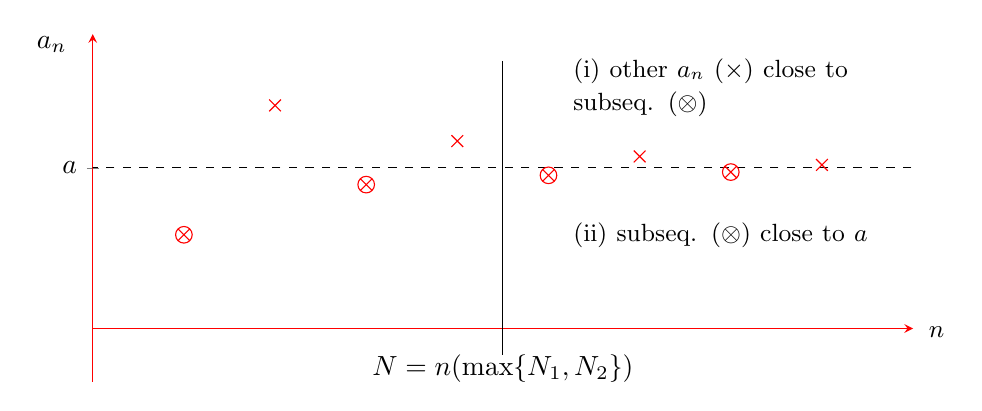
\begin{tikzpicture}
\begin{axis}[
 axis line style={red},
axis lines=middle,
     x label style={at={(axis description cs:1.05,0.1)}},
     y label style={at={(axis description cs:-0.08,1.02)}},
    xlabel={\small $n$},
    ylabel={$a_n$},
  ymin =-0.2,
  ymax = 1.1,
  xmin = 1,
  xmax = 10,
     ytick = {0.6},
   yticklabels={$a$},
   xtick = 0,
  width=12cm,height=6cm]
   \addplot[samples at={3,5,7,9}, only marks, mark=x,  mark options={red}, mark size=3pt]{1/x+0.5};
    \addplot[samples at={2,4,6,8},only marks, mark options={red},mark=otimes,mark size=3pt]{-1/(x^2)+0.6};
       \draw[dashed] (axis cs:20,0.6) -- (axis cs:0,0.6); %a line
            \draw (axis cs:5.5,1) -- (axis cs:5.5,-0.1) node  at (axis cs:5.5,-0.15) {$N =n(\mathrm{max}\{N_1,N_2\})$}; %N line
                  \node[text width=4cm] at (axis cs:8,0.9) {\small (i) other $a_n$ ($\times$) close to subseq. ($\otimes$)};
          \node[text width=4cm] at (axis cs:8,0.35) {\small (ii) subseq. ($\otimes$) close to $a$};
            
  \end{axis}
\end{tikzpicture}
\end{center}

Set $N = n(\mathrm{max}\{N_1,N_2\}) \geq \mathrm{max}\{N_1,N_2\} \geq N_1$. Then $\forall n \geq N$ we have
\[\begin{aligned}|a_n - a| &= |(a_n - a_N) + (a_N - a)| \\
&\leq |a_n - a_N| + |a_N - a|\\
 &< \epsilon + \epsilon = 2\epsilon	
\end{aligned}\]\end{proof}\vspace*{5pt}


\textbf{Aside:} Fix $c >0$. Then $a_n \to a$ iff 
\[\boxed{\forall \epsilon >0,~\exists N_{\epsilon} \iN \text{ s.t. } n \geq N_\epsilon \implies |a_n - a| < c\epsilon (*)}\]
Ex: Show $\implies$

\begin{proof}[Proof $\impliedby$] Fix $\epsilon >0$. Set $e' = \epsilon/c >0$. Then $(*) \implies $
\[\exists N_\epsilon \iN \text{ s.t. } n \geq N_\epsilon \implies |a_n - a| < c\epsilon' = \epsilon\qedhere\]
\end{proof}

\textbf{Beware!} Do not let $c$ depend on $\epsilon$ (Nor $N!$), e.g. if we let $c = \frac{1}{\epsilon}$ then $(*)$ becomes $\forall \epsilon >0,~\exists N \iN$ s.t. $\forall n \geq N,~|a_n - a| < 1$ and $a_n = \frac{1}{2} \forall n,~ a = 0$ satisfies this!\\

We can also go the other way round: Cauchy theorem $\implies$ BW. 

\begin{proof}[Proof 2 of BW]



Take a bounded sequence $(a_n)$. We want to find a convergent subsequence. 

Given $a_n \in [-R,R]~ \forall n$, repeatedly subdivide to make this interval smaller. So either
\begin{enumerate}
\item $\exists$ infinite number of $a_n$'s in $[-R,0]$
\item $\exists$ infinite number of $a_n$'s in $[0,R]$
\end{enumerate}

Pick one of these intervals with inifnite number of $a_n$'s; call it $[A_1,B_1]$, length $2R/2$. 

Now subdivide again; call $[A_2,B_2]$ one of the intervals $[A_1,\frac{A_1+B_1}{2}]$ or $[\frac{A_1+B_1}{2},B_1]$ with infinitely many $a_n$'s in it with length $2R/2^2$ etc. 

We get a sequence of intervals $[A_n,B_n]$ of length $2R/2^n$ each containing an infinite number of $a_n$s which are nested: $[A_{k+1},B_{k+1}] \subseteq [A_k,B_k]$


Now we use a \emph{diagonal argument}. Let $b_i = a_{n(i)}$ be an elements of the sequence in $[A_i,B_i]$ s.t. $n(i) > n(i-1)$. (This is possible because $\exists$ infinite no. of elements of sequence in $[A_i,B_i]$. 

 \textbf{Claim:} $b_i = a_{n(i)}$ is convergent.

Fix $\epsilon >0$. Take $N_{\epsilon} > \frac{2R}{\epsilon}$, so that $\frac{2R}{2^{N_{\epsilon}}} < \frac{2R}{N_{\epsilon}} < \epsilon$. Then $\forall i, j \geq N_{\epsilon}$ we have
\[|b_i - b_j| < \frac{2R}{2^{N_{\epsilon}}} < \epsilon\]
beacause $b_i,b_j \in [A_{N_{\epsilon}},B_{N_{\epsilon}}] \implies (b_i)$ Cauchy $\implies$ convergent.
	\end{proof}\vspace*{5pt}
	

%!TEX root = M1P1.tex

\pagebreak

\sektion{Series}\vspace*{5pt}

\begin{definition}\lecturemarker{9}{5 Oct}
An (infinite) series is an expression \[\displaystyle{\sum_{n=1}^{\infty} a_n} \text{ or } a_1  + a_2 + \dots \] where $(a_i)_{i\geq 1}$ is a sequence.
\end{definition}

\subsektion{Convergence of Series}

\begin{definition}
We say that the series $\sum a_n = A \in \mathbb{R}$ (or ``converges to $A \in \RR$'') iff the sequence of partial sums $S_n:= \sum_{i=1}^n a_i \in \RR$ converges to $A \in \RR$; $S_n \to A$ as $n \to \infty$. 
\end{definition}



\[
\begin{tikzcd}[row sep=1.5cm]
 &  \mbox{Sequence of partial sums $(s_n)$}\arrow[<->]{dr}{s_n = \sum_{i=1}^n a_i} \\ 
\mbox{Sequence $(a_n)$} \arrow[<->]{ur}{a_n = s_n - s_{n-1}} \arrow[<->]{rr}{\text{Equivalent Information}} && \mbox{Series $\sum a_n$}
\end{tikzcd}
\]~\\



\begin{example}
$a_n = x^n,~n \geq 0$. Consider $\sum_{n=0}^{\infty} a_n = \sum_{n=0}^{\infty} x^n$.

Define $s_n = \sum_{i=0}^n x^i = 1 + x + \dots + x^n$ then $xS_n = x + \dots + x^n + x^{n+1} \implies S_n - xS_n = 1 - x^{n+1}$
\[\implies S_n = \begin{cases}
 \frac{1-x^{n+1}}{1-x} & x \neq 1\\
 n+1 & x = 1	
 \end{cases}
\]
So for $|x| < 1$, we see that 
\[S_n = \frac{1}{1-x} - \frac{x^{n+1}}{1-x} \to \frac{1}{1-x} \text{ as } n \to \infty\]

(Question Sheet 3: proves that $r^n \to 0$ if $|n| < 1$)
\end{example}\vspace*{5pt}

So we have proved that $(s_n)$ is convergent and $\sum x^n = \frac{1}{1-x} \iR$ for $|x| < 1$. 

For $|x| \geq 1$, $a_n = x^n$ does not $\to 0$ as $n \to \infty$. So $\sum a_n = \sum x^n$ is \emph{not} a real number (does not converge) by the following result:\\


\begin{theorem}
$\sum_{n=0}^\infty a_n$ is convergent $\implies a_n \to 0$	
\end{theorem}

\begin{proof}
$S_n - S_{n-1} = a_n$. If $S_n \to S$ then $S_{n-1} \to S$ (Ex). So by the algebra of limits $a_n$ is convergent and $\lim_{n\to \infty} a_n = \lim_{n\to\infty} S_n - \lim_{n\to \infty} S_{n-1} = S - S = 0$.	
\end{proof}

\begin{proof}[Proof from first principles]
Fix $\epsilon >0$. $s_n \to s$, so 
\[\exists N\iN \text{ s.t. } \forall n \geq N,~|s_n - s| < \epsilon\]
\[\begin{aligned}
\implies |a_n| &= |s_n - s_{n-1}| \\
&\leq |s_n - s| + |s_{n-1} - s| \\ 
&< \epsilon + \epsilon \text{, for } n-1 \geq N.	
\end{aligned}
\]
So $\forall n \geq N+1$, $|a_n| < 2\epsilon$. 
\end{proof}\vspace*{5pt}

\begin{remark}
Converse is \emph{not} true. E.g. $a_n = \frac{1}{n} \to 0$, but $\sum \frac{1}{n}$ is \emph{not} convergent. 	
\end{remark}~

\begin{example}
$\displaystyle{\sum_{n=1}^{\infty} \frac{1}{n^2}}$ is convergent\footnote{Famously to $\pi^2/6$ - see \href{https://en.wikipedia.org/wiki/Basel_problem}{Basel Problem}.} 	

\begin{proof}(Trick) First do $\sum_{n=1}^\infty \frac{1}{n(n+1)}$ and use $\frac{1}{n(n+1)} = \frac{1}{n} - \frac{1}{n+1}$

\[\begin{aligned}
S_n &= \sum_{i=1}^n \frac{1}{i} - \frac{1}{i+1} \\
&= \textstyle{(1-\frac{1}{2}) + (\frac{1}{2} - \frac{1}{3}) + \dots + (\frac{1}{n} - \frac{1}{n+1})}\\
&= 1 - \frac{1}{n+1} \to 1 \text{ as } n \to \infty	
\end{aligned}
\]

$\implies \sum_{n=1}^\infty \frac{1}{n(n+1)}$ is convergent to $1$.

Ao now compare the partial sums $\sigma_n$ of $\sum \frac{1}{n^2}$ to those of $\sum \frac{1}{n(n+1)} = 1$

\[\begin{aligned}
\sigma_n = \sum_{i=1}^n \frac{1}{i^2} &= 1 + \sum_{j=1}^{n-1} \frac{1}{(j+1)^2} \\
&\leq 1 + \sum_{j=1}^{n-1}\frac{1}{j(j+1)}\\
&= 1 + s_{n-1}	
\end{aligned}
\]

$s_{n-1}$ is a bounded (by $1$) monotonically increasing sequence (because $\frac{1}{n(n+1)} >0$), convergent to $1$. So $s_{n-1} < 1~\forall n \implies \sigma_n < 2 \implies$ bounded above monotonic increasing sequence $\implies \sigma_n$ is convergent $\implies \sum \frac{1}{n^2}$ is convergent.	
\end{proof}
\end{example}\vspace*{5pt}


Similarly $\sum \frac{1}{n^k}$ is convergent for $k \geq 2$ because $\frac{1}{n^k} \leq \frac{1}{n^2}$. In fact $\zeta(k) = \sum \frac{1}{n^k}$ is convergent for $k \in (1,\infty)$... See later!\\


\begin{theorem}[Algebra of Limits for Sequences]

If $\sum a_n = A \iR$ and $\sum b_n = B \iR$, then $\sum (\lambda a_n + \mu b_n) = \lambda A + \mu B \iR$. 
\end{theorem}

Put differently, if $\sum a_n$, $\sum b_n$ converge, then so does $\sum (\lambda a_n + \mu b_n)$ and it equals $\lambda \sum a_n + \mu \sum b_n$. 


\begin{proof}
Partial sums (to $n$ terms) of $\sum (\lambda a_n + \mu b_n)$ is 
\[\sum_{i=1}^{n} (\lambda a_i + \mu b_i) = \lambda \sum_{i=1}^{n} \lambda a_i + \sum_{i=1}^{n} \mu b_i \to \lambda \sum_{i=1}^{\infty} a_n + \mu \sum_{i=1}^{\infty} \mu b_n \]
as $n \to \infty$ by the algebra of limits for sequences. So the partial sums converge.
\end{proof}~



\lecturemarker{10}{5 Oct}
\begin{theorem}[Comparison Test]
If $0 \leq a_n \leq b_n$ and $\sum_{n=1}^{\infty} b_n$ converges, then $\sum_{n=1}^{\infty} a_n$ converges.	 (and $0 \leq \sum_{n=1}^{\infty}a_n \leq \sum_{n=1}^{\infty}b_n$)
\end{theorem}

\begin{proof}
Call the partial sums $A_n$, $B_n$ respectively. Then
\[0 \leq A_n \leq B_n \leq \sum_{i=1}^{\infty} b_i = \lim_{n\to \infty}B_n\]	

So $A_n$ is bounded and monotonically increasing $\implies$ convergent.
 
(Question Sheet 3 shows that if $A_n \leq B_n$ and $A_n \to A$, $B_n \to B$, then $A \leq B$)
\end{proof}\vspace*{5pt}


\begin{proposition}
Suppose $a_n \geq 0 ~\forall n$. Then $\sum_{n=1}^{\infty} a_n$ converges iff $S_N = \sum_{n=1}^{N}a_N$ is bounded above and $\sum_{n=1}^{\infty} a_n$ diverges to $\infty$ (i.e. $S_n \to +\infty$ as $N \to \infty$) iff $S_N = \sum_{n=1}^{N} a_n$ is an unbounded sequence. 
\end{proposition}

\begin{proof}
$a_n \geq 0 \iff (S_n)$ is monotonic increasing. So $(S_n)$ bounded $\iff$ convergent.

$S_N$ unbounded $\iff \forall R>0,~ \exists N \in \NN$ such that $\forall n \geq N,~ S_n > R \iff S_n \to +\infty$. 
\end{proof}\vspace*{5pt}

Exercise: (Converse of Comparison Test)
If $0 \leq a_n \leq b_n$ then $\sum a_n$ diverges to $\infty\implies \sum b_n$ diverges to $\infty$\\


\begin{example}
$\sum_{n=1}^{\infty} \frac{1}{n^{\alpha}},~ \alpha > 1$ is convergent.
\begin{proof}
(Trick!) Arrange the partial sum as follows:
\[\begin{aligned}
1 + \frac{1}{2^\alpha} + \frac{1}{3^\alpha} + \dots  = 1 + \left(\frac{1}{2^\alpha} + \frac{1}{3^\alpha}\right) &+ \left(\frac{1}{4^\alpha} + \dots +\frac{1}{7^\alpha}\right)  \\ 
&+ \left(\frac{1}{8^\alpha} + \dots + \frac{1}{15^\alpha}\right) \\
&+ \left(\frac{1}{16^\alpha} + \dots + \frac{1}{31^\alpha}\right) \\
&+ \dots  \end{aligned}\]
Note that the $k$th bracketed term:
\[\left(\frac{1}{(2^k)^\alpha} + \dots +\frac{1}{(2^{k+1}-1)^\alpha}\right ) \leq \frac{1}{2^{k\alpha}} + \dots + \frac{1}{2^{k\alpha}} = \frac{2^k}{2^{k\alpha}} = \frac{1}{2^{k(\alpha-1)}}\]

So any partial sum is less than some finite sum of these bracketed terms, i.e. for some sufficiently large $N$: \[ S_N < \sum_{k=0}^{N} \frac{1}{2^{k(\alpha -1)}} = \frac{1-\frac{1}{2^{(N+1)(\alpha -1)}}}{1-\frac{1}{2^{(\alpha-1)}}} \leq \frac{1}{1-\frac{1}{2^{\alpha-1}}}\] because $\alpha >1$, so $\left|\frac{1}{2^{\alpha-1}}\right| < 1$, so denominator $>0$. 

So partial sums are bounded above $\implies$ convergent. 
\end{proof}	
\end{example}~

\begin{definition}
Say that the series $\sum_{n=1}^{\infty}a_n$ is \emph{absolutely convergent} if and only if the series $\sum_{n=1}^{\infty} |a_n|$ is convergent	
\end{definition}~

\begin{example}
$\sum_{n=1}^{\infty} \frac{(-1)^{n+1}}{n}$ is \emph{not} absolutely convergent, but it is convergent.


\textit{Rough Working.} $1 - \frac{1}{2} + \frac{1}{3} - \frac{1}{4} + \frac{1}{5} - \frac{1}{6} + \dots = (1-\frac{1}{2}) + (\frac{1}{3} - \frac{1}{4}) + (\frac{1}{5} -\frac{1}{6}) + \dots$, the $k$th bracket $\frac{1}{2k-1} - \frac{1}{2k} = \frac{1}{2k(2k-1)}$. This is positive and $\leq \frac{1}{2k(2k-2)} = \frac{1/4}{k(k-1)}$, seen earlier sum of these is convergent.

So cancellation between consecutive terms is enough to make series converge by comparison with $\sum \frac{1}{k(k-1)}$.

\begin{proof}
Fix $\epsilon >0.$ Then use 2 things\begin{enumerate}
\item[(1)] $\sum \frac{1}{2k(2k-1)}$	is convergent
\item[(2)] $\frac{(-1)^{n+1}}{n}\to 0$
\end{enumerate}
By (1) $\exists N_1$ such that $\forall n \geq N_1,~ \sum_{n=1}^{\infty} \frac{1}{k(k-1)} < \epsilon$

By (2) $\exists N_2$ such that $\forall n \geq N_2,~ \left|\frac{(-1)^{n+1}}{n}\right| < \epsilon$

Set $N =$ max$(N_1,N_2)$. Then $\forall n \geq N$, we have:
\[S_n = \left(1-\frac{1}{2}\right) + \left(\frac{1}{3} - \frac{1}{4}\right) + \dots \left(\frac{1}{2j-1} - \frac{1}{2j} \right) + \delta = \sum_{k=1}^{j} \frac{1}{2k(2k-1)} + \delta\] 
where $\delta = \begin{cases}
 	\frac{(-1)^{n+1}}{n} & \text{ if } n \text{ is odd.}\\
 	0 & \text{ if } n \text{ is even.}
 \end{cases}
$ $~~\left(j = \lfloor \frac{n}{2} \rfloor\right)$   $j = \begin{cases}
 	\frac{n-1}{2} & \text{ if } n \text{ is odd.}\\
 	\frac{n}{2} & \text{ if } n \text{ is even.}
 \end{cases}
$
\[\implies S_n = \sum_{k=1}^{\infty} \frac{1}{2k(2k-1)} - \sum_{k=\lfloor \frac{n}{2} \rfloor + 1}^{\infty} \frac{1}{2k(2k-1)} + \delta\]
\[\text{So } \left|S_n - \sum_{k=1}^{\infty} \frac{1}{2k(2k-1)} \right| \leq \sum_{k=\lfloor \frac{n}{2} \rfloor + 1}^{\infty} \frac{1}{2k(2k-1)} + \frac{1}{n} < \epsilon + \epsilon\] for all $n \geq 2N$ (so that $\lfloor \frac{n}{2} \rfloor + 1 >N$) 
\end{proof}
\end{example}\vspace*{10pt}

\lecturemarker{11}{5 Oct}
\begin{theorem}
	If $(a_n)$ is absolutely convergent, then it is convergent.
\end{theorem}

\begin{proof}
Let $S_n = \sum_{i=1}^{n} |a_i|$, $\sigma+n = \sum_{i=1}^n a_i$ be the partial sums.

We're assuming that $S_n$ converges. Therefore $S_n$ is Cauchy: 
\[ \forall \epsilon >0~ \exists N_{\epsilon}\text{ such that }n > m \geq N_{\epsilon} \implies |S_n - S_m| < \epsilon \iff |a_{m+1} + \dots + |a_n| < \epsilon\]
i.e. the terms in the tail of the series contribute little to the sum 

$\implies |a_{m+1} + \dots + a_n| < \epsilon$ by the triangle inequality $\implies |\sigma_n - \sigma_m| < \epsilon \implies (\sigma_n)$ is Cauchy $\implies \sum a_i$ is convergent.
\end{proof}\vspace*{5pt}

\begin{example}
$\sum_{n=1}^{\infty} z_n$ is convergent for $|z| < 1$, divergent for $|z| \geq 1$
\begin{proof}
$\sum_{n=1}^{\infty} z_n$ is absolutely convergent because we showed that $\sum_{n=1}^{\infty} |z|^n$ converges to $\frac{1}{1 - |z|}$ for $|z| < 1$	

For $|z| \geq 1$, the individual terms $z^n$ have $|z^n| \geq 1$, so $z^n \not\to 0$, so $\sum z^n$ divergent.
\end{proof}
\end{example}


\subsektion{$*$Re-arrangement of Series$*$}
\emph{This section was non-examinable in 2015}

\textbf{Beware.} Do not rearrange series and sum them in a different order unless you can prove the result is the same.\\

\begin{example}
$\sum (-1)^{n+1} = 1 - 1 + 1 - 1 + \dots$

either this $``=" (1-1) + (1-1) + \dots = 0$

or this $``=" 1 - (1-1) + (1-1) + \dots = 1$	
\end{example}

A better (convergent) example\\

\begin{example}
$a_n:= 1 - \frac{1}{2} + \frac{1}{3} - \frac{1}{4} + \dots 	= \log 2$

(See later for proof of result, it's the series for $\log(1+x) = x - \frac{x^2}{2} + \dots$ putting $n=1$, which is on our radius of convergence!)

Reorder the sum as follows:
\[\begin{array}{cccccccc}
	1 & ~ & +\frac{1}{3} & ~ & +\frac{1}{5} & ~ & +\frac{1}{7} & \dots \\
	& -\frac{1}{2} & ~ & -\frac{1}{4} & ~ & -\frac{1}{6} & ~ & \dots \\
	&&&&&&&\\
= 	1 & ~ & +\frac{1}{3} & ~ & +\frac{1}{5} & ~ & +\frac{1}{7} & \dots \\
	-\frac{1}{2} [& 1 & ~ & +\frac{1}{2} & ~ & +\frac{1}{3} & ~ & \dots ]\\

\end{array}\]
Terms with even denominator appear only in bottom row ($\times -\frac{1}{2}$)

Terms with odd denominator appear in the top row ($\times 1$) + bottom row $\times -\frac{1}{2} \implies (\times \frac{1}{2})$ in total. 

So $a = \frac{1}{2}[1-\frac{1}{2} + \frac{1}{3} - \frac{1}{4} + \frac{1}{5} -\frac{1}{6} + \dots] \implies a = a/2,~\cont$ (But clearly $a \geq \frac{1}{2} > 0$)

\end{example}

This happened because when I reordered I went along the bottom row twice as fast as I went along the top row. Since the top and bottom row diverges to $\infty$, I'm computing $\infty - \infty$, and originally I did this like $(a+n) - n$ as $n \to \infty$. Now I'm doing it like $(a + n) - (n + \frac{a}{2})$ as $n \to \infty$. 


In fact I can rearrange the sum to converge to anything I like.\\

\begin{example}
Rearrange $a_n = \dfrac{(-1)^{n+1}}{n} \to 42$. 

We reorder the sum as follows
\begin{enumerate}
\item Take only off terms $a_{2n+1} > 0$ until their sum is $>42$. We can do this as $1 + \frac{1}{3} + \dots$ diverges to $\infty$!
\item Now take only even terms $a_{2n} < 0$ until sum gets $<42$
\item Repeat (i) and (ii) to fade.
\end{enumerate}


We can do each step because $\sum a_{2n+1}$ diverges to $\infty$ and $\sum a_{2n}\to -\infty$. We use all the terms eventually (so this is really a reordering of the whole sum)

Why? If not then we must eventually only take terms of one type (w.l.o.g. the even -ve terms) but these sum to $-\infty,~\cont$. At point they reach $<42$ we switch back to odd +ve terms.

Finally proof that the reordered sum converges to $42$ 
\[a_n \to 0 \text{ so }\forall \epsilon >0,~\exists N \iN \text{ s.t. } n \geq N \implies |a_n| < \epsilon ~(*)\]

So now we go to a point in the reordering where we have used all $a_i$ up to $N$ and then further to the point where the partial sum crosses $42$. At this point, $(*)$ holds, so I'm within $\epsilon$ of $42$. from this point on the sum is always within $\epsilon$ of $42$ by design and by $(*)$. 

\[\implies |s_n - 42| < \epsilon \text{ from this point on}\qed\]
\end{example}


More generally \lecturemarker{12}{9 Feb}
 if $(a_n)$ is a sequence whose terms tend to zero, $a_n \to 0$ and such that:\vspace*{5pt}
 \quad 
 $\bullet \displaystyle{\sum_{\substack{n \text{ s.t.} \\a_n \geq 0}} a_n}$ diverges ($\to \infty$) \quad 
 $\bullet \displaystyle{\sum_{\substack{n \text{ s.t.}\\ a_n < 0}}  a_n}$ diverges ($\to -\infty$)	
 
 then I can rearrange the series $\sum a_n$ (1) to make it converge to \emph{any} number I like $\iR$ or (2) to  make it diverge to $\infty$ or (3) to $-\infty$. 
 
 For (1), the Algorithm is same as for $\sum \frac{(-1)^n}{n}$	
 \begin{enumerate}
 \item Pick +ve terms until partial sums are $>$ my fixed real number, $a$
 \item Now pick -ve terms until partial sum is $< a$
 \item Go back to (i) and repeat.
 \end{enumerate}\vspace*{5pt}
 
 If however $a_n \to 0$ and \vspace*{5pt}
 
   $\bullet \displaystyle{\sum_{\substack{n \text{ s.t.} \\a_n \geq 0}} a_n} \to \infty$\quad 
 $\bullet \displaystyle{\sum_{\substack{n \text{ s.t.}\\ a_n < 0}}  a_n}$ converges
 
 Then however I rearrange $\sum a_n$ it will always diverge to $+ \infty$~\\
 
 Similarly if $a_n \to 0$ and \vspace*{5pt}
 
 	$\bullet \displaystyle{\sum_{\substack{n \text{ s.t.} \\a_n \geq 0}} a_n}$ converges
 \quad $\bullet \displaystyle{\sum_{\substack{n \text{ s.t.}\\ a_n < 0}}  a_n} \to -\infty$ 
 
 $\implies  \sum a_n$ diverges to $-\infty$ (however rearranged)\\

\textbf{ Final case:} $a_n \to 0$ and 

 	$\bullet \displaystyle{\sum_{\substack{n \text{ s.t.} \\a_n \geq 0}} a_n}$ converges
 \quad $\bullet \displaystyle{\sum_{\substack{n \text{ s.t.}\\ a_n < 0}}  a_n}$ converges

This is the \emph{good case} where \emph{however} you rearrange, $\sum a_n$ is \emph{absolutely convergent} to the same limit, $\sum_{a_n \geq 0} a_n + \sum_{a_n < 0} a_n$. 
We will prove this next time.\\

\begin{remark} Rearrange partial sums only. $a+ b = b+a$ is fine. Infinite sums are tricky!	
\end{remark}\vspace*{5pt}


\begin{definition}[Rearrangement of a Sequence] 
	If $M: \NN \to \NN$ is a bijection (i.e. a reordering!) then define $b_m:= a_{M(m)}.$ Then $(b_m)_{m \geq 1}$ is a rearrangement of $(a_n)$.
\end{definition}

e.g. if $M(1), M(2), M(3), M(4),\dots$ is $5,1,6,2,\dots$ then $b_1,b_2,b_3,b_4,\dots$ is $a_5,a_1,a_6,a_2,\dots$.\\


\begin{theorem}
Suppose that $\sum a_n$ is absolutely convergent. Then
\begin{itemize}
\item[(1)] $\sum_{a_n \geq 0} a_n$ is convergent to $A$ (say)	
\item[(2)] $\sum_{a_n < 0} a_n$ is convergent to $B$ (say)	
\item[(3)] $\sum a_n = A+B$
\item[(4)] $\sum b_m = A+B$ where $(b_m)$ is any rearrangement of $(a_n)$
\end{itemize}
\end{theorem}

\begin{proof} \lecturemarker{13}{9 Feb}
Key Idea: $\sum |a_n|$ is convergent so has a small ``tail'', so by the triangle inequality $\sum a_n$ has an even smaller tail so should converge. 

But what to? No idea, so we use the Cauchy criterion! 

(1) $s_n = \sum_{i=1}^n a_i,~\sigma_n = \sum_{i=1}^n |a_i|$. $\sigma_n$ convergent $\implies \sigma_n$ is Cauchy. 
\[\forall \epsilon > 0~\exists N \iN \text{ s.t. } \forall n,m \geq N,~|\sigma_n - \sigma_m | < \epsilon\]
w.l.o.g. $n \geq m$, this says 
\[\sum_{i=m+1}^n |a_i| < \epsilon \implies \left|\sum_{i=m+1}^m a_i \right| < \epsilon \iff |s_n - s_m| < \epsilon\]

So $(s_n)$ is Cauchy $\implies s_n$ is convergent. 

(2) $\sum_{a_n \geq 0} a_n$ is also convergent because the partial sums are monotonic increasing, bounded above by $\sum |a_n|$. Similarly $\sum_{a_n < 0} a_n$ is decreasing, $\geq -\sum |a_n|$, so also cvgt. 

(3) Let $A = \sum_{a_n \geq 0} a_n$ and $B = \sum_{a_n < 0} a_n$. Then $\forall \epsilon >0$
\[\exists N_1 \text{ s.t. } n \geq N_1 \implies \left| \sum_{a_n \geq 0}^{\text{first } n \text{ terms}} - A\right| < \epsilon \]
\[\exists N_2 \text{ s.t. } n \geq N_2 \implies \left| \sum_{a_n < 0}^{\text{first } n \text{ terms}} - B\right| < \epsilon \]

Let $N$ be max$(I,J)$ where $I$ is the $N_i$th $a_i \geq 0$ (the $N_i$th positive term) and $a_J$ the $N_J$th -ve term. Then $\forall n \geq N$

\[\begin{aligned}\left|\sum_{i=1}^n - (A+B)\right| 
&\leq \left|\sum_{a_i \geq 0}^n a_i - A\right| + \left|\sum_{a_i < 0}^n a_i - B\right| < \epsilon + \epsilon = 2\epsilon 
\end{aligned}
\]
So $\sum_{i=1}^n \to A+B$ as $n \to \infty$.\\

(4) Finally $(b_m)$ is a rearrangement of $(a_n)$. We want to show that $\sum b_m$ converges to $A+B$ as well. 

Pick $M \iN$ such that $b_1,b_2,\dots,b_M$ contains all of $P_1,P_2,\dots,P_I$ and $N_1,N_2,\dots,N_J$ where $P_i$ is the $i$th $a_i \geq 0$ and $N_J$ is the $j$th $a_j <0$. 

[i.e. we're far enough down the rearranged series to have included all significant $a_i \geq 0$ and $a_i <0$ which sum to $<\epsilon$ by (1) and (2)]

Then $\forall m \geq M$ we have

\[\begin{aligned}
\left|\sum_{i=1}^m b_i - (A+B)\right| 
&\leq \left|\sum_{b_i \geq 0}^m b_i - A\right| + \left|\sum_{b_i < 0}^m b_i - B\right|\\
&\leq \left|\sum_{a_k \geq 0}^I a_k + \delta - A\right| + \left|\sum_{a_k < 0}^J a_k +\delta' - B\right|\\
&< \epsilon + \epsilon = 2\epsilon 
\end{aligned}
\]
(where $\delta =$ sum of $a_k \geq 0$ with $k >I$ and $\delta' =$ sum of $a_k < 0$ with $k > J$) \end{proof}

\subsektion{Tests for convergence}

\setcounter{equation}{4}
We already met the first test:
\begin{theorem}[Comparison I]
If $0 \leq a_n \leq b_n$ and $\sum_{n=1}^{\infty} b_n$ converges, then $\sum_{n=1}^{\infty} a_n$ converges.	 (and $0 \leq \sum_{n=1}^{\infty}a_n \leq \sum_{n=1}^{\infty}b_n$)
\end{theorem}

Recall proof from earlier: $s_n = \sum a_i$ is monotonic increasing and bounded above by $\sum b_i \in \RR$.\\

\setcounter{equation}{17}
\begin{theorem}[Comparison II - Sandwich Test]
	Suppose $c_m \leq a_n \leq b_n$ and $\sum c_n,~\sum b_n$ are both convergent. Then $\sum a_n$ is convergent.
\end{theorem}
\begin{proof}
Use Cauchy. $\forall \epsilon >0,~ \exists N \in \NN$ such that $\forall n,m > N$
\[\left|\sum_{i=m+1}^n b_i\right| < \epsilon,~\left|\sum_{i=m+1}^n c_i\right| < \epsilon\] since the partial sums of $b_i,~c_i$ are Cauchy. Therefore
\[-\epsilon <\sum_{i=m+1}^n c_i \leq \sum_{i=m+1}^n a_i \leq \sum_{i=m+1}^n b_i < \epsilon   \]
\[\implies \left|\sum_{i=1}^{n} a_i - \sum_{i=1}^m a_i\right| < \epsilon \implies \left(\sum_{i=1}^{n} a_i \right) \text{ is Cauchy.} \qedhere\]
\end{proof}\vspace*{5pt}

 \lecturemarker{14}{12 Feb}
\begin{theorem}[Comparison III]
If $\frac{a_n}{b_n}\to l \in \RR$ then $\sum b_n$ absolutely convergent $\implies \sum a_n$ is absolutely convergent.
\end{theorem}
\begin{proof}
Pick $\epsilon = 1$, then $\exists N \in \NN$ such that $\forall n \geq N$:
\[\left|\frac{a_n}{b_n} - l \right| < 1 \implies \left|\frac{a_n}{b_n}\right| < |l| + 1 \implies |a_n| < (|l| + 1)|b_n|\]
So now by the comparison test $\sum_{n \geq N} |b_n|$ convergent $\implies \sum_{n \geq N} |a_n|$ convergent $\implies \sum_{n\geq 1} |a_n|$ convergent. 	
\end{proof}

We have used the obvious fact that if $\sum_{n \geq N} c_n$ is convergent then $\sum_{n \geq 1} c_n$ is also convergent (and vice-versa). Exercise: prove this!\\

\begin{theorem}[Alternating Series Test.]
Given an alternating sequence $a_n$ where $a_{2n} \geq 0$, $a_{2n+1} \leq 0~ \forall n$. Then $|a_n|$ monotonic decreasing to $0 \implies \sum a_n$ convergent
\end{theorem}

\begin{proof}
Write $a_n = (-1)^nb_n,~b_n\geq 0 ~\forall n	$. Consider the partial sums $S_n = \sum_{i=1}^{n} (-1)^nb_n$.\\

  Observe that: \begin{enumerate}
 \item[(1)]$S_i \leq S_{2n}~\forall i \geq 2n$
 \item[(2)]$S_i \geq S_{2n+1}~\forall i\geq 2n+1$
 \end{enumerate}
 Since if $i=2j$ is even, then
  \[\begin{aligned}
	S_{2j} &= S_{2n} + a_{2n+1} + \dots + a_{2j}\\ 
	&= S_{2n} + \underbrace{(-b_{2n+1} + b_{2n+2})}_{\leq 0} + \dots + \underbrace{(-b_{2j-1} + b_{2j})}_{\leq 0} \leq S_2n
\end{aligned}
\]
 
  If $i= 2j+1$ is odd, then similarly:
   \[\begin{aligned}
	S_{2j} = S_{2n} + \underbrace{(-b_{2n+1} + b_{2n+2})}_{\leq 0} + \dots + \underbrace{(-b_{2j-1} + b_{2j})}_{\leq 0} - b_{2j+1} \leq S_2n
\end{aligned}
\]
  
 So now $\forall \epsilon >0,~ \exists N \in \mathbb{N}$ such that $\forall n \geq N,~|b_n| < \epsilon$. So $\forall n,m\geq 2n$, we have: \[S_{2N+1} \leq S_n,~S_m \leq S_{2N}\] 
 \[\begin{aligned}\text{So } |S_n - S_m| &\leq |S_{2N+1} - S_{2N}|\\
 &= b_{2n+1} < \epsilon	
\end{aligned}
\]
\end{proof}\vspace*{5pt}

\begin{theorem}[Ratio Test]
If $a_n$ is a sequence such that $\left|\frac{a_{n+1}}{a_n}\right| \to r < 1$, then $\sum a_n$ is absolutely convergent.	
\end{theorem}
\begin{proof}
Fix $\epsilon = \frac{1-r}{2} > 0$. Then $\exists N \in \mathbb{N}$ such that $\forall n \geq N$
\[\left|\frac{a_{n+1}}{a_n} - r\right| < \epsilon \implies |a_{n+1}| < (r + \epsilon)|a_n|\]
Set $\alpha := r + \epsilon = \frac{1 + r}{2} < 1$. 

Inductively
\[|a_{N+m}| < \alpha|a_{N+m-1}| < \dots < \alpha^m|a_N|\]	
So $\forall k \geq N$ \[|a_k| <  \alpha^{k-N}|a_N| = C\alpha^k\]

Then \[C\sum_{k=N}^{n} \alpha^k = \frac{C(\alpha^N-\alpha^n)}{1-\alpha} \to \frac{C'}{1-\alpha} \text{ as } n \to \infty \text{, since } \alpha < 1\]

So by the comparison test $\sum_{k\geq N} |a_k|$ is convergent $\implies \sum_{k\geq 1} |a_k|$ is convergent
\end{proof}

The point is that the ratio test, when it applies, says that $a_n \approx r^n$ i.e. decays exponentially. But many convergent series like $\sum \frac{1}{n^2}$ do not decay so fast.\\

\begin{example}
$a_n = \dfrac{100^n(\cos n\theta + i\sin n\theta}{n!} = \dfrac{(100e^{i\theta})^n}{n!}$

Then 
\[\left|\frac{a_{n+1}}{a_n}\right| = \frac{(100e^{i\theta})^{n+1}/(n+1)!}{(100e^{i\theta})^{n}/n!} = \frac{100}{n+1} \to 0\]
So by the ratio test, $\sum a_n$ is absolutely convergent $\implies \sum a_n$ is convergent.	
\end{example}\vspace*{5pt}

 \lecturemarker{15}{16 Feb}
\begin{theorem}[Root Test]
If $\lim_{n\to \infty} |a_n|^{1/n} = r < 1$, then $\sum a_n$ is absolutely convergent.	
\end{theorem}
\begin{proof}
Fix $\epsilon = \frac{1-r}{2} > 0$. Then $\exists N \in \mathbb{N}$ such that $\forall n \geq N$
\[\left||a_n|^{1/n} - r\right| < \epsilon \implies |a_n|^{1/n} < r + \epsilon\]
Set $\alpha := r + \epsilon = \frac{1 + r}{2} < 1$, so that $|a_n| < \alpha^n$. Then
\[ \sum_{k=1}^n\alpha^k = \frac{\alpha(1-\alpha^n)}{1-\alpha}  \to \frac{\alpha}{1-\alpha} \text{ as } n \to \infty \text{ since } \alpha < 1\]

So by the comparison test $\sum_{k\geq 1} |a_k|$ is convergent.
\end{proof}


\subsektion{Power Series}\vspace*{10pt}
\begin{theorem}[Radius of Convergence]
	Consider the series $\sum a_nz^n ~(*),~ z,a_n \iC$. 
	
	Then $\exists R \in [0,\infty]$ such that $|z| < R \implies (*)$ is aboslutely convergent, $|z| > R \implies (*)$ divergent
\end{theorem}

\begin{proof}
Define $R =$ sup $S = \{|z| : a_nz^n \to 0\}$	 or $R = \infty$ if the set is unbounded. (1) Suppose $|z| < R$. $|z|$ not an upperbound for $S \implies \exists w$ such that $|w| > |z|$ and $a_nw^n \to 0.$ Then \[|a_nz^n| = |a_nw^n|\left|\frac{z}{w}\right|^n \leq A\left|\frac{z}{w}\right|^n\] Since $\left|\frac{z}{w}\right| < 1 \implies \sum|a_nz^n|$ cvgt. Similarly $|z| >R  \implies$ $\sum |a_nz^n|$ divergent. 

(2) Suppose $|z| > R$. Then $a_nz^n \not\to 0$ as $n \to \infty \implies \sum a_nz^n$ does not converge.
\end{proof}\vspace*{5pt}

\begin{clicker}
What is the radius of convergence for $\sum \frac{z^n}{n}$? 

\textbf{Answer:} $R = 1$, in fact the series
\begin{enumerate}
\item $\sum z^n$
\item $\sum \frac{z^n}{n}$
\item $\sum \frac{z^n}{n^2}$	
\end{enumerate}
all have this $R$.

\begin{proof}
The ratio test gives  $\left|\dfrac{z^{n+1}}{z^n}\cdot f(n)\right|$ where $f$ is a rational function of $n$ of degree $0$. $= |zf(n)| \to |z|$ as $n \to \infty$. So convergent for $|z| < 1$ and divergent for $|z| > 1$.  	
\end{proof}

But notice different behaviours on $|z| = 1$. \begin{enumerate}
 \item Never converges on $|z| = 1$ as $z^n \not\to 0$
 \item Convergent for some $|z| = 1$ (in fact $z \neq 1$), divergent for others
 \item Also convergent $\forall z$ with $|z|  =1$ (comparison with $\sum \frac{1}{n^2}$)	
 \end{enumerate}
\end{clicker}\vspace*{5pt}


\subsubsektion{Products of Series}
Consider 
\[\begin{aligned}
\sum_{n=0}^{\infty} a_nz^n \sum_{n=0}^{\infty}b_nz^n &= (a_0 + a_1z + a_2z^2 + \dots) (b_0 + b_1z + b_2z^2 + \dots)\\
&``='' a_0b_0 + (a_0b_1 + a_1b_0)z + (a_0b_2 + a_1b_1 + a_2b_0)z^2 + \dots \\
&= \sum_{n=0}^{\infty} c_nz^n 	
\end{aligned}
\]
where $c_0 = a_0b_0$, $c_1 = a_0b_1 + a_1b+0, \dots c_n = a_0b_n + a_1b_{n-1} + \dots + a_nb_0$. 

So we set $c_n = \sum_{i=0}^{n} a_i b_{n-i}$ and ask when is the product $\sum a_nz^n \sum b_nz^n$ equal to $\sum c_nz^n$? We can also do this without the $z^n$'s:\\

\begin{definition}
Given series $\sum a_n,~\sum b_n$, their \emph{Cauchy Product} is the series $\sum c_n$ where $c_n := \sum_{i=0}^n a_ib_{n-i}$.	
\end{definition}\vspace*{5pt}

  \lecturemarker{16}{19 Feb}
\begin{theorem}[Cauchy Product]
If $\sum a_n, \sum b_n$ are absolutely convergent, then $\sum c_n$ is absolutely convergent to $(\sum a_n) \cdot (\sum b_n)$	
\end{theorem}
\textit{Proof.}
See handout on blackboard. Non-examinable. \\

\begin{corollary}
If $\sum A_nz^n$ and $\sum B_nz^n$ have radius of convergence $R_A$ and $R_B$ respectively, then $\sum c_nz^n$ has radius of convergence $R_C \geq \mathrm{min}\{R_A,R_B\}$.	
\end{corollary}
\begin{proof}
By the previous theorem, for $|z| < \mathrm{min}\{R_A,R_B\} ~(*)$ we have $\sum A_nz^n$ and $\sum B_nz^n$ absolutely convergent $\implies \sum c_nz^n$ absolutely convergent to their product. 

In fact $|c_nz^n| \to 0$ so $|z| < R_c$. So by $(*)$, $R_c \geq \mathrm{min}\{R_A,R_B\}$.
\end{proof}~

\begin{example}
$\sum z^n$ has $R_A = 1$, $1-z$ has $R_B = \infty$ So their cauchy product $\sum c_nz^n$ has $R_c \geq 1$. 

\emph{Ex:} Check $c_0 = 1, c_n = 0~\forall n \geq 1$, so in fact $R_c = \infty$	.

But we only know that $\sum c_n z^n = 1 = (\sum z^n)(1-z)$ when $|z| < 1 = \mathrm{min}\{R_A,R_B\}$. 
\end{example}\vspace*{5pt}

\subsubsektion{Exponential Power Series}\vspace*{5pt}

\begin{definition}[Exponential Series]
\[E(z):= \sum_{n=0}^\infty \frac{z^n}{n!},~z\iC\]

Ratio test: $|a_{n+1}/a_n| = \frac{z}{n+1} \to 0$ as $n \to \infty ~\forall z \iC\implies E(z)$ is absolutely convergent $\forall z\iC$.  
\end{definition}\vspace*{5pt}

\begin{proposition}
$E(z)E(w) = E(z + w)$
\end{proposition}
\begin{proof}
By Cauchy product theorem
\[E(z)E(w) = \sum_{n=0}^\infty c_n\]
where $c_n = \sum_{i=0}^n \dfrac{z^i}{i!}\dfrac{w^{n-i}}{(n-i)!} \implies c_n = \dfrac{(z+w)^n}{n!}$.
\end{proof}\vspace*{5pt}

\begin{corollary}
$E(z) \neq 0$ and $\dfrac{1}{E(z)} = E(-z)$
\end{corollary}
\begin{proof}
$E(z)E(-z) = E(0) = 1$.	
\end{proof}\vspace*{5pt}

\begin{definition}
$e:= E(1) = \sum \frac{1}{n!} \in (-0,\infty)$	
\end{definition}\vspace*{5pt}

\begin{corollary}
$E(n) = e^n$ for $n \iN$	
\end{corollary}
\begin{proof}
	$E(n) = E(1 + (n-1)) = E(1)E(n-1) = \dots = (E(1))^n$.
\end{proof}\vspace*{5pt}

\begin{proposition}
$E(q) = e^q$ for $q \iQ$ (recall rational powers of $a \iR$ were defined in M1F)	
\end{proposition}
\begin{proof}
	Suppose $q > 0$; write $q = \frac{m}{n}$, $m,n \iN$. Then 
	\[\textstyle{E(q) = E(\underbrace{\frac{1}{n} + \dots + \frac{1}{n}}_{n \text{ times}}) = E(\frac{1}{n})^m}\]
	But \[E(\frac{1}{n})^n = E(\underbrace{\frac{1}{n} + \dots + \frac{1}{n}}_{m \text{ times}}) = E(1) = e\]
	
	\[ \implies E(\frac{1}{n}) = e^{1/n}\text{ and }E(q) = E(\frac{1}{n})^m = e^{m/n} = e^q\]
	
	If $q = \frac{-m}{n}$ then $E(q) = 1/E(m/n) = \frac{1}{e^{m/n}} = e^{-m/n} = e^q$.
\end{proof}

So we know that $E(x) = e^x ~\forall x \iQ$. Later we define $e^x~\forall x\iR$ by \emph{continuity} and we will show $E(x)$ is also continuous and so $E(x) = e^x~\forall x\iR$. \\
 
 
Some \lecturemarker{17}{20 Feb} useful properties of $E(x)$:
\begin{enumerate}
\item $x \geq 0 \implies E(x) \geq 1$ and $x > 0 \implies E(x) > 1$ (obvious from series)
\item $E(x) > 0~\forall x \iR$
\item $E(x)$ is strictly increasing for $x\iR$: $x < y \implies E(y) = E(x)E(y-x) > E(x).1$
\item $|x| < 1$ then $|E(x) - 1| < \frac{|x|}{1-|x|}$
\item $\RR \ni x \mapsto E(x)$ is a continuous bijection onto $(0,\infty)$. (proven later)
\item So we can define $\log: (0,\infty) \to \RR$ as inverse of $E$, i.e. $y = \log x$ defined by $\iff x = e^y$ with the usual log properties
\end{enumerate}~

We can also define $a^x$ for $a \in(0,\infty),x\in \RR$ by $a^x = E(x\log a)$

Exercise: If $x \iQ$ this agrees with Corti's definition. 

And trig functions $\cos \theta = \Re E(i\theta)$, $\sin \theta = \Im E(i\theta)$ etc. 

Exercise: $E(i\theta + i\phi) = E(i\theta)E(i\phi)$ implies what?
	




\sektion{Continuity}

\subsektion{Continuity and Limits}
\begin{definition}
	Given a function $f: \RR \to \RR$, we say that $f$ is \emph{continuous at $a \iR$} if and only if 
	\[\forall \epsilon >0, ~\exists \delta >0 \text{ such that } |x-a| < \delta \implies |f(x) - f(a)| < \epsilon \]
\end{definition}

So $\delta$ depends on $a, \epsilon$. ``Once $x$ is close to $a$, then $f(x)$ is close to $f(a)$''.

More precisely: ``However close (i.e. within $\epsilon$) I want $f(x)$ to be to $f(a)$, I can arrange it by taking $x$ close (i.e. within $\delta$) to $a$''.


\begin{center}
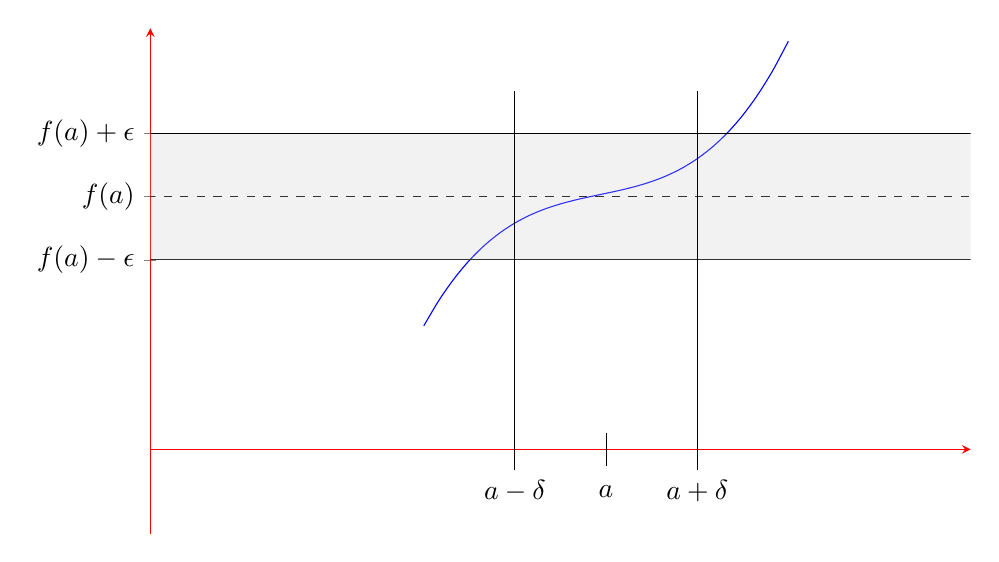
\begin{tikzpicture}
\begin{axis}[
 axis line style={red},
 axis lines=middle,
   %  x label style={at={(axis description cs:1.05,0.4)}},
   %  y label style={at={(axis description cs:-0.08,1.02)}},
  ymin = -0.2,
  ymax = 1,
  xmin = 1,
  xmax = 10,
     ytick = {0.75, 0.45,0.6},
   yticklabels={$f(a) + \epsilon$,$f(a) -\epsilon$, $f(a)$},
   xtick = 0,
  width=12cm,height=8cm]
   \addplot[draw=blue, domain=4:8,smooth] {(0.0309*x^3 - 0.5504*x^2 + 3.313*x - 6.13)};
       \draw (axis cs:20,0.75) -- (axis cs:0,0.75); %fa+e line
      \draw (axis cs:20,0.45) -- (axis cs:0,0.45); %fa-e line
       \draw[dashed] (axis cs:20,0.6) -- (axis cs:0,0.6); %fa line
         \fill[gray!40,nearly transparent] (axis cs:0,.45)-- (axis cs: 0,0.75) -- (axis cs: 10,0.75) -- (axis cs: 10,0.45) -- cycle;
            \draw (axis cs:5,0.85) -- (axis cs:5,-0.05) node at (axis cs:5,-0.1) {$a-\delta$};
                        \draw (axis cs:6,0.04) -- (axis cs:6,-0.04)  node at (axis cs:6,-0.1) {$a$};
                        \draw (axis cs:7,0.85) -- (axis cs:7,-0.05) node at (axis cs:7,-0.1) {$a + \delta$};
  \end{axis}
\end{tikzpicture}
\end{center}


Equivalently: $\forall \epsilon > 0,~ \exists \delta >0 \text{ such that } |f(x) - f(a)| < \epsilon ~ \forall x \text{ with } |x-a| < \delta$\\

Or: $\forall \epsilon > 0, ~ \exists \delta > 0 \text{ such that } f(a- \delta, a + \delta) \subseteq (f(a)- \epsilon, f(a) + \epsilon)$

Where $S\subseteq R$ then $f(S)$ is the set $\{f(x):x \in S\}$\\

Or: $\forall \epsilon,~\exists \delta >0 \text{ such that } f^{-1}(f(a) - \epsilon, f(a) + \epsilon) \supseteq (a - \delta, a + \delta)$

Where $f: A \to B \subset T$ then $f^{-1}(T) = \{a \in A:f(a) \in T\}$ [Don't need $f^{-1}$ to exist !!]\\


\begin{example}
\[f(x) = \begin{cases}
 0 & x \leq 0 \\
 1 & x > 0	
 \end{cases}
\]	 Then $f$ is not continuous at $x = 0$

\begin{proof}
Take $\epsilon = 1$ (or $0 < \epsilon < 1$). Then if $f$ is continuous at $x = 0$ we know that $\exists \delta > 0$ such that $|f(x) - f(0)| < 1~ \forall x \in (0 - \delta, 0 + \delta)~(*)$. In particular, take $x = \delta/2$ to find that $|1-0| < 1$ by 	$(*)$.
\end{proof}
\end{example}

``Jump discontinuity'' is another type of discontinuity\\


\begin{example}
\[f(x) = \begin{cases}
 \sin(\frac{1}{x}) & x \neq 0\\
 r & x = 0	
 \end{cases}
\] Then $f$ is discontinuous at $x = 0$ (for any $r$).	

\begin{center}
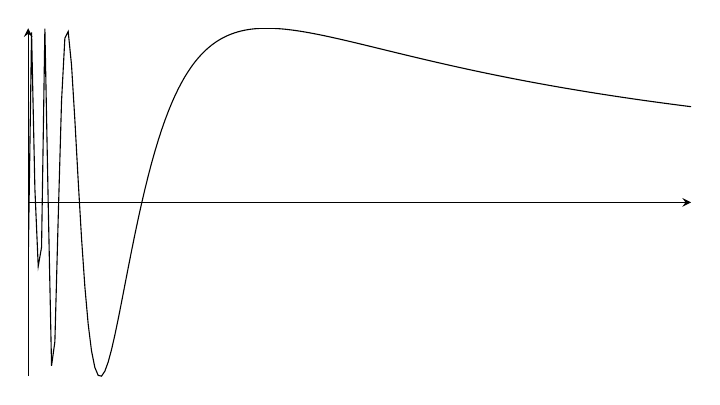
\begin{tikzpicture}
\begin{axis}[
axis lines=middle,
xtick = 0,
ytick = 0,
  width=10cm,height=6cm]
   \addplot[domain=0.0005:0.03,samples=200]{sin(1/x)};
 \end{axis}
\end{tikzpicture}
\end{center}

\emph{Idea of proof}: If $f$ is continuous at $x = 0$, then $f(x) \in (r-\epsilon, r + \epsilon)$ is close to $f(0) = r$ for $x \in (- \delta, \delta).$ In particular, $f(x)$ and $f(y)$ are close to each other (within $2\epsilon$). But $f(x)$ could be $+1$ and $f(y)$ could be $-1$, $\cont$.
\begin{proof}
Fix $\epsilon \in (0,1]$. If $f$ is continuous at $0$, then $\exists \delta > 0$ such that $|f(x) - f(0)| < \epsilon~\forall x \in (\delta,\delta)$. In particular, $\forall x,y \in (-\delta, \delta), |f(x) - f(y)| < 2\epsilon \leq 2$, by the triangle inequality. 

Now choose $n \in \mathbb{N}$, $n > \frac{1}{\delta}$. Then take $x = \frac{1}{(4n+1)\pi/2} \in (0,\delta)$, $y = \frac{1}{(4n+3)\pi/2} \in (0,\delta)$. Then 
\[|\sin(1/x) - \sin(1/y)| = |1 - (-1)| = 2 ~\cont\qedhere\]
\end{proof}

\end{example}~


\begin{example}
\lecturemarker{18}{5 Oct}
$f: \RR \to \RR$, $f = mx + c$ is continuous at $a, ~\forall a \iR$. 

\emph{Rough working:} We want 
\[\begin{aligned}|f(x) - f(a)| < \epsilon &\iff |(mx+c) - (ma + c)|  < \epsilon \\
&\iff |mx(-a)| < \epsilon\\
&\iff |x-a| < \frac{\epsilon}{|m|} \text{ if } m \neq 0 \\
&\impliedby |x-a| < \frac{\epsilon}{|m|+1} 
\end{aligned}
\]
So set $\delta:= \epsilon / (1 + |m|)$. Then $|x-a| < \delta \implies |f(x) - f(a)| < \epsilon$
\begin{proof}
Set $\delta:= \frac{\epsilon }{1 + |m|} > 0$. Then when $|x-a| < \delta$ we have  
\[\begin{aligned}
|(mx+ c) - (ma +c)| &= |f(x) - f(a)| \\
&= |m||x-a| \\
&< |m|\delta = \epsilon \frac{|m|}{|m|+1} < \epsilon	
\end{aligned}\]
\end{proof}
\end{example}

\begin{example}
$f: \RR\to \RR, f(x) = x^2$
Proposition: $f$ continuous on $\RR$ (i.e. at $a,~\forall a \iR$)

\emph{Rough working:} 
\[|f(x) - f(a)| = |x^2-a^2| = |x+a||x-a|\]
we want this to be $< \epsilon$, i.e. $|x-a| < \frac{\epsilon}{|x+a|} *(*)$

But we can't let $\delta$ depend on $x$!!

\textbf{Problem:} If $|x-a| < \frac{\epsilon}{R} \forall R>0$, then $|x-a| =0$.

\textbf{Solution:} I only care about $x$ close to $a$; within $1$ say.


So, so long as I choose $\delta \leq 1$, then I know that 
\[|x-a| < \delta \implies |x+a| \leq |x-a| + 2|a| \leq 1 + 2|a|\]
So now $|x-a| < \dfrac{\epsilon}{1 + 2|a|} \implies (*)$

So to ensure both conditions we set $\delta = \mathrm{min}\{1,\epsilon/(1+2|a|)\}$

\begin{proof}
Fix $\epsilon >0$, $a \iR$. Set $\delta = \mathrm{min}\{1,\frac{\epsilon}{1 + 2|a|}\}$. Then $|x-a| < \delta \implies$
\begin{enumerate}
\item $|x-a| < 1 \implies |x+a| < 1 + 2|a|$
\item $|x-a| < \dfrac{\epsilon}{1 + 2|a|}$
\end{enumerate}

\[\implies |x^2 -a^2| = |x-a||x+a| < \dfrac{\epsilon}{1+2|a|}\cdot(1+2|a|) = \epsilon\]
\end{proof}
\end{example}~

\begin{clicker}
Fix $a,b \iR$. Then $x < a \implies x < b$ tells us? 

\textbf{Answer:} $a \geq b$. 

Prove that $f(x) = \begin{cases}
 	\frac{1}{x} & x \neq 0\\
 	0 & x = 0
 \end{cases}$
 is discontinuous at $x = 0$

Student answer:
\begin{enumerate}
\item Suppose $f$ is cts at $0$
\item Then $\forall \epsilon >0,~\exists \delta > 0$ s.t.
\item $|x| < \delta \implies |f(x) - f(0)| = |1/x| < \epsilon$
\item $\implies |1/(x/2)| = |2/x| < 2\epsilon$
\item But $|x| < \delta \implies |x/2| < \delta$ so
\item should get that $|f(x/2) - f(0)| = |1/(x/2)| < \epsilon$
\item This contradicts $(*)$	
\item So $f$ is not continuous at $0$
\end{enumerate}

\textbf{Answer:} (vii) is the problem. (vi) $\implies$ (iv) doesn't contradict (iv).
\end{clicker}


Notice 
\lecturemarker{19}{5 Oct} the definition of continuity makes sense whenever I have a notion of distance.  e.g. in $\RR^n$ use $|\vec{x} - \vec{y}| := \sqrt{\sum_{i=1}^n (x_i - y_i)^2}$.\\

\begin{definition}
$f: \RR^n \to \RR^m$ is continuous at $a \in \RR^n$ iff 
\[\forall \epsilon >0,~\exists \delta >0 \text{ s.t. } |\vec{x} - \vec{a}| < \delta \implies |f(\vec{x}) - f(\vec{a})| < \epsilon\]	
\end{definition}

\textbf{Notation:} The $\epsilon$-ball around $\vec{a}\in\RR^n$ is $B_\epsilon(\vec{a}) := \{\vec{x} \in \RR^n |\vec{x} - \vec{a}| < \epsilon\}$

So if $n = 1$, $B_\epsilon(a) = (a-\epsilon, a + \epsilon) \subseteq \RR$. 

Using this we can rewrite our definition of continuity:\\

\begin{definition}
$f: \RR^n \to \RR^m$ is continuous at $\vec{a} \in \RR^n$ iff 
\[\forall \epsilon > 0,~\exists \delta > 0 \text{ s.t. } f(B_\delta(\vec{a})) \subseteq B_\epsilon(f(\vec{a}))\]	
\end{definition}

So every point within $\delta$ of $\vec{a}$ gets mapped by $f$ to within $\epsilon$ of $f(\vec{a})$, equivalently 
\[\boxed{\forall \epsilon > 0,~\exists \delta > 0 \text{ s.t. } B_\epsilon(\vec{a}) \subseteq f^{-1}(B_\epsilon(f(\vec{a})))}\]


\begin{center}
\includegraphics[width = 12cm]{ball1.jpg}
\end{center}


$f^{-1}(B_\epsilon(f(\vec{a}))) := \{\vec{x} \in \RR^n : f(\vec{x}) \in B_\epsilon (f(\vec{a}))\}$

Continuity at $\vec{a}$ says that $\vec{a}$ is in the ``interior'' of $f^{-1}(B_\epsilon (f(\vec{a})))$, i.e. $\exists$ a small ball $B_\delta (\vec{a})$ around it which is also in $f^{-1}(B_\epsilon(f(\vec{a})))$. 

So continuity at $\vec{a} \iff$ If $\vec{x}$ moves a tiny bit around $\vec{a}$ then $f(\vec{x})$ moves a tiny bit around $f(\vec{a})$.\pagebreak

\begin{example}
$f(x) = \begin{cases}
 	x\sin 1/x & x \neq 0\\
 	0 & x = 0
 \end{cases}$

\begin{center}
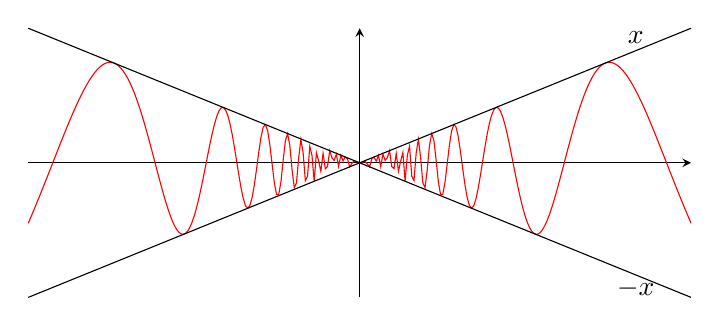
\begin{tikzpicture}
\begin{axis}[
axis lines=middle,
xtick = 0,
ytick = 0,
  width=10cm,height=5cm]
   \addplot[color = red, domain=-0.003:0.003,samples=300]{x*sin(1/x)};
   \addplot[domain=-0.003:0.003,smooth]{x};
   \addplot[domain=-0.003:0.003,smooth]{-x};
   \draw node at (axis cs: 0.0025,0.0028) {$x$};
   \draw node at (axis cs: 0.0025,-0.0028) {$-x$};
 \end{axis}
\end{tikzpicture}
\end{center}


\begin{proposition}
$f$ is continuous at $0$	
\end{proposition}

\begin{proof}
Fix $\epsilon >0$. Then 
\[|f(x) - f(0) = |x\sin\frac{1}{x}| \leq |x|\]
Take $\delta = \epsilon$. Then $|x| < \delta \implies |x| < \epsilon \implies |f(x) - f(0)| < \epsilon$	
\end{proof}
\end{example}\vspace*{5pt}

\begin{proposition}
$E: \CC \to \CC$ defined by $E(z) := \sum_{n=0}^{\infty} \frac{z^n}{n!}$ is continuous (i.e. continuous at $a,~\forall a \iC$)	
\end{proposition}
[Ex: from this show that $x \mapsto \sin x$ is continuous on $\RR$]

\emph{Rough working:} 
\[\begin{aligned}
|E(z) - E(a)| &= |E(a)(E(z-a)-E(0))| \\ 	
&= |E(a)| |E(z-a) -1|\\
& \leq |E(a)| \cdot \frac{|z-a|}{1-|z-a|}
\end{aligned}
\]
for $|z-a| < 1$ (see earlier lecture)
\[\begin{aligned}
\text{We want this to be } < \epsilon &\iff |z-a| < \frac{\epsilon}{|E(a)|}(1-|z-a|)\\
&\iff (1 + \epsilon/|E(a)|)|z-a| < \frac{\epsilon}{|E(a)|}\\
&\iff |z-a| < \epsilon/|E(a)|/(1 + \epsilon/|E(a)|)
\end{aligned}
\]


\begin{proof}
Fix $\epsilon >0$. Set $\delta = \dfrac{\epsilon}{|E(a)| + \epsilon} ~(*)$

Then we calculate that 
\[\begin{aligned}
|E(z) - E(a)| &\leq |E(a)| \frac{|z-a|}{1-|z-a|} \\
&< |E(a)| \cdot \frac{\delta}{1-\delta}	
\end{aligned}
\]	
for all $z$ with $|z-a| < \delta$. But by $(*)$, $\dfrac{\delta}{1-\delta} = \dfrac{\epsilon}{|E(a)|}$. 

So $|z-a|< \delta \implies |E(z) - E(a)| < \epsilon$.
\end{proof}


\begin{theorem}
$f,g: \RR \to \RR$ cts at $a \in \RR \implies (f + g), f\cdot g$ are cts at $a$.
\end{theorem}
\begin{proof}
	Fix $\epsilon >0.$ \[\exists \delta_1 >0 \text{ such that }|x-a| < \delta_1 \implies |f(x) - f(a)| < \epsilon\] and\[\exists \delta_2 >0 \text{ such that }|x-a| < \delta_1 \implies |g(x) - g(a)| < \epsilon\]
	 Set $\delta =$ min$\{\delta_1,\delta_2\}.$ Then $\forall x$ such that $|x-a| < \delta:$
	\[|(f+g)(x) - (f+g)(a)| \leq |f(x) - f(a)| + |g(x) - g(a)| < 2\epsilon\]
	
	For (2): Similarly
	\[|f(x)g(x) - f(a)g(a)| \leq |g(x)||f(x) - f(a)| + |f(a)||g(x) - g(a)| ~(*)\]
	
	We need a bound on $|g(x)|$. We cannot bound $g(x)~ \forall x$!  But near $a$, $g(x)$ is close to $g(a)$, so we can bound $g(x)$ near $a$
	
	Take $\epsilon =1$ 
	\[\exists \delta_1 > 0\text{ s.t. }|x-a| < \delta_1 \implies |g(x) - g(a)| < 1 \implies |g(x)| < 1 + |g(a)| ~(A)\]
	
	Now fix any $\epsilon >0$. Then 
	\[\exists \delta_2 > 0\text{ s.t. }|x-a| < \delta_2 \implies |f(x) - f(a)| < \epsilon/1+|g(a)| ~ (B)\] (to cancel $|g(x)| < 1+|g(a)|$ in $(*)$)
	
	\[\exists \delta_3 > 0 \text{ s.t. } |x-a| < \delta_3 \implies |g(x) - g(a)| < \frac{\epsilon}{1 + |f(a)|}~ (C)\]
	(to cancel $|f(a)|$ in $(*)$)
	
	Set $\delta := \mathrm{min}\{\delta_1,\delta_2,\delta_3\}$. Then $|x-a| < \delta \implies (A), (B), (C)$ all hold. 
	
	Substitute into $(*)$ to find 
	\[\begin{aligned}|f(x)g(x) - f(a)g(a)| &< 1+|g(a)|\frac{\epsilon}{1+|g(a)|} + |f(a)|\frac{\epsilon}{1 + |f(a)|}\\
	&\leq \epsilon + \epsilon = 2\epsilon
\end{aligned}\]
\end{proof}


\begin{theorem}
	$f:\RR \to \RR$ cts at $a \in \RR$, $g:\RR \to \RR$ cts at $f(a) \in \RR$, then $g \circ f$ cts at $a$
\end{theorem}

\emph{Idea of Proof:} We want $g(f(x))$ to be close (within $\epsilon$) to $g(f(a))$. 

But $g$ is continuous at $f(a)$! So sufficient for $f(x)$ to be close (within $\delta_g$ to $f(a)$. But $f$ is continuous at $a$! so we can arrange this (by taking $\epsilon = \delta_g$ by taking $x$ to be close (within $\delta_g$) to $a$. 

\begin{proof}\lecturemarker{20}{5 Oct}
Fix $\epsilon >0.$ $g$ is continuous at $f(a)$, so \[\exists \delta > 0\text{ s.t. }|g - f(a)| < \delta \implies |g(y) - g(f(a))| < \epsilon\]

Also $f$ is continuous at $a$, so 
\[\exists \eta > 0\text{ s.t. }|x-a| < \eta \implies |f(x) - f(a)| < \delta\]

\noindent Hence $|x-a| < \eta \implies |f(x) - f(a)| < \delta \implies |g(f(x)) - g(f(a))| < \epsilon.$
\end{proof}

\begin{corollary}
$a^x:= E(x\log a), ~a>0$ is continuous $\forall x \iR$	
\end{corollary}
\begin{proof}
It is a composition $\displaystyle{\RR \xrightarrow[x \mapsto x\log a]{} \RR \xrightarrow[y \mapsto E(y)]{} \RR }$ of two functions.	
\end{proof}

Exercise: Show $\sin 1/x$ is continuous for $\RR\backslash\{0\} \to \RR$. (i.e. show $1/x$ is continuous from first principles, $\sin x$ is continuous using continuity of $E(x)$ and compose!)\vspace*{15pt}

\begin{example}
Suppose $f:\RR\to \RR\backslash\{0\}$ is continuous. Then $1/f$ is continuous. 

\begin{proof}
Pick $a\iR$. Show $1/f(x)$ is continuous at $a$: 

\[\left|\frac{1}{f(x)} - \frac{1}{f(a)}\right|  = \frac{1}{|f(x)f(a)|}|f(x)-f(a)| ~(*)\]

We need to bound $f(x)$ below! Need $|f(x)| > \text{ some }\eta > 0 \iff \frac{1}{|f(x)|} < \frac{1}{\eta}$

We can't, but we can near $a$! $f(a) \neq 0$, so take $\epsilon' = |f(a)|/2 >0$. Then 
\[\exists \delta' \text{ s.t. } |x-a| < \delta' \implies|f(x) - f(a)| < \epsilon' = \frac{|f(a)|}{2}\]
\[\implies |f(x)| > |f(a)| -\epsilon = \frac{|f(a)|}{2}\]


\[\begin{aligned}
\text{So by } (*) \text{, we have }\left|\frac{1}{f(x)} - \frac{1}{f(a)}\right| &< \frac{1}{|f(a)|/2\cdot |f(a)|} |f(x) - f(a)| \\ 
	& = \frac{2}{|f(a)|^2}|f(x) - f(a)|
\end{aligned}
\]

Fix $\epsilon >0$. Set $\epsilon'' = \mathrm{min}\left(\frac{|f(a)|}{2}, \frac{\epsilon}{2}|f(a)|^2\right) > 0$

Then $\exists \delta > 0$ such that $|x-a| < \delta \implies |f(x) - f(a)| < \epsilon''$ (by continuity of $f$ at $a$)

$\implies (1) |f(x)| > |f(a)| - \epsilon'' \geq |f(a)| - |f(a)|/2$ and $(2) |f(x) - f(a)| < \frac{\epsilon}{2}|f(a)|^2$. So 

\[\begin{aligned}
\left|\frac{1}{f(x)} - \frac{1}{f(a)}\right| &= \frac{1}{|f(x)||f(a)|} |f(x) -f(a)| \\
&< \frac{1}{|f(a)|/2\cdot|f(a)|}\cdot \frac{\epsilon}{2}|f(a)|^2 = \epsilon	\qedhere
\end{aligned}
\]
\end{proof}	
\end{example}


\begin{theorem}
	$f: \RR \to \RR$ is cts at $a \in \RR$ iff $\forall$ sequences $x_n \to a$, $f(x_n) \to f(a)$
\end{theorem}

In one direction this is somewhat easy: if $x_n \to a$ and $f$ is continuous at $a$, then $f(x_n)$ gets close to $f(a0$ as $x_n$ gets close to $a \implies f(x_n) \to f(a)$. 

The converse is \emph{much harder}. If I want to see if $f$ is continuous, I can test with a sequence $x_n \to a$ to see if $f(x_n)$ if close to $f(a)$ when $n$ is large. But $x_n$'s doesn't cover all $x$'s! But if I use \emph{all} sequences $x_n \to a$ then I do cover all $x$ and get a theorem. 

\begin{proof}
If $f$ is cts at $a$, fix $\epsilon >0$. $\exists \delta > 0$ such that $|x-a| < \delta \implies |f(x) - f(a)| < \epsilon$. Now $x_n \to a$, so $\exists N \in \mathbb{N}$ such that $n \geq N \implies |x_n - a| < \delta \implies |f(x_n) - f(a)| < \epsilon$.\\

\noindent Suppose $f$ is not cts at $a\in \RR$ for contradiction.

 Then $\exists \epsilon >0$ such that $\forall \delta >0,~\exists x \in (a-\delta,a+\delta)$ such that $|f(x) -f(a)| \geq \epsilon.$ 
 
 Choose $\delta = \frac{1}{n}$. $\exists x_n \in (a - \frac{1}{n},a + \frac{1}{n})$ such that $|f(x_n) - f(a)| \geq \epsilon$. 
 
 So $|x_n-a| < \frac{1}{n}~\forall n \implies x_n \to a$. But $f(x_n) \centernot\implies f(a),~\cont$.  
\end{proof}\vspace*{5pt}

\begin{example}
$f(x) =\begin{cases}
\sin 1/x & x \neq 0\\
0 = 0
\end{cases}
$	

This is \emph{not} continuous at $0$. But if we take $x_n \to 0$, then $f(x_n) = \sin(n\pi) = 0~\forall n$, so $f(x_n)\to f(0)$. so this sequence does not defect. 

Have to choose a different sequence e.g. $x_n = \frac{2}{\pi},\frac{2}{3\pi},\frac{2}{5\pi},\dots,$ gives $\sin\frac{1}{x_n} = (-1)^{n+1} \not\to f(0) \implies f$ discontinuous at $0$.  
\end{example}

To get this problem of sequences not covering the whole of an interval $(a-\delta, a+\delta)$ (so having to consider all sequences at once - nasty), we can let $x$ run through all of $\RR$ with the following definition:\\

\begin{definition}\lecturemarker{21}{5 Oct}
$f: \RR\to \RR$, $a\iR$. 

We say that $f(x) \to b$ as $x \to a$ (or ``$\lim_{x\to a} f(x) = b$'') iff 
\[\forall \epsilon >0,~\exists \delta > 0 \text{ s.t. } 0 < |x-a| < \delta \implies |f(x) - b| < \epsilon\]	
\end{definition}

``$x$ close to $a$ (but not equal!!) $\implies f(x)$ close to $b$''\vspace*{15pt}

\begin{example}
$f(x) = \begin{cases}
 0 & x \neq 0\\
 1 & x=0	
 \end{cases}$
	
Then $\lim_{x\to 0} f(x) = 0$

e.g. We can talk about $\lim_{x\to 0}f(x)$ for $f: \RR\backslash\{0\} \to \RR$.
\end{example}

\begin{theorem}
$f: \RR \to \RR$ is continuous at $a \iR$ iff $f(x) \to f(a)$ as $x \to a$	
\end{theorem}

\begin{proof}
$f$ is continuous at $a\iR$ says (1):
\[\forall \epsilon > 0,~\exists \delta > 0 \text{ s.t. } |x-a| < \delta \implies |f(x) - f(a)| < \epsilon\]

Whereas $f(x) \to f(a)$ as $x \to a$ says (2):
\[\forall \epsilon > 0,~\exists \delta > 0 \text{ s.t. } 0 < |x-a| < \delta \implies |f(x) - f(a)| < \epsilon\]

So (1)$\implies$ (2).

Suppose (2). Then I get (1) except for when $|x-a| = 0$. But when $|x-a| = 0$, then $x=a$, so $f(x) = f(a)$, so $|f(x) - f(a)| < \epsilon$, so I still get (1).
\end{proof}


Can extend the definition of continuity to functions defined on subsets of $\RR$ or $\RR^n$ e.g.\vspace*{10pt}
\begin{definition}
$f: S \to \RR^m$, $S \subseteq \RR^n$, is continuous at $\vec{a} \in S$ iff
\[\forall \epsilon > 0,~\exists \delta > 0 \text{ s.t. } (0 < |\vec{x}-\vec{a}| < \delta \text{ and } x \in S) \implies |f(\vec{x}) - f(\vec{a})| < \epsilon\]
\end{definition}\vspace*{5pt}

\begin{example} 
$f: \RR \to \RR$, $f(x) = \begin{cases}
 0 & x \iQ\\
 1 & x \not\in\QQ	
 \end{cases}$
 
 This is discontinuous. But $\left.f\right|_\QQ: \QQ \to \RR$ is continuous. 	
\end{example}

Related to this is one-sided continuity:\\

\begin{definition}
$f: \RR \to \RR$ is \emph{right continuous} at $a\iR$ iff
\[\forall \epsilon > 0,~\exists \delta > 0 \text{ s.t. } x \in [a, a+\delta) \implies |f(x) - f(a)| < \epsilon\]
\end{definition}

Exercise: $f$ is right continuous at $a \in \RR \iff \left. f \right|_{[a,\infty)}: [a,\infty) \to \RR$ is continuous at $a \in \RR$. 

Exercise: $f: \RR \to \RR$ is continuous at $a\iR \iff f$ is both right and left continuous at $a \iR$\\

\begin{definition}
	$f(x) \to b$ as $x \to a_+$ ``as $x$ tends to $a$ from above''
	means 
	\[\forall \epsilon > 0,~\exists \delta > 0 \text{ s.t. } x \in (a,a+\delta) \implies |f(x) - f(a)| < \epsilon\]
\end{definition}

Exercise: Just as before find that $f$ is right continuous at $a\iff f(x) \to f(a)$ as $x \to a_+$

\pagebreak
\subsektion{Intermediate Value Theorem}\vspace*{5pt}

\begin{theorem}[Intermediate Value Theorem] If $f: [a,b] \to \RR$ cts, $c \in (f(a),f(b)),$ then $\exists x \in [a,b]$ such that $f(x) = c$
\end{theorem}

\begin{center}
\begin{tikzpicture}
\begin{axis}[
 axis line style={red},
 axis lines=middle,
   %  x label style={at={(axis description cs:1.05,0.4)}},
   %  y label style={at={(axis description cs:-0.08,1.02)}},
  ymin = -0.2,
  ymax = 1,
  xmin = 1,
  xmax = 10,
     ytick = {0.5},
   yticklabels={$c$},
   xtick = 0,
  width=12cm,height=6.5cm]
   \addplot[draw=blue, domain=4:5,smooth] {(0.0309*x^3 - 0.5504*x^2 + 3.313*x - 6.23)};
      \addplot[draw=blue, domain=7:8,smooth] {(0.0309*x^3 - 0.5504*x^2 + 3.313*x - 6.23)};
       \draw[dashed] (axis cs:20,0.5) -- (axis cs:0,0.5); %c line
                        \draw (axis cs:6,0.04) -- (axis cs:6,-0.04)  node at (axis cs:6,-0.1) {$x$};
                     \draw (axis cs:4,0.04) -- (axis cs:4,-0.04)  node at (axis cs:4,-0.1) {$a$};
                        \draw (axis cs:8,0.04) -- (axis cs:8,-0.04)  node at (axis cs:8,-0.1) {$b$};

  \end{axis}
\end{tikzpicture}
\end{center}


If $f$ is continuous it must cross the line $y=c$ at some point $x \in [a,b]$. 

\begin{corollary}
Any odd degree polynomial over $\RR$ has a root $\iR$	
\end{corollary}
\begin{proof}
w.l.o.g. $p(x) = x^{2n+1} + a_{2n}x^{2n} + \dots + a_1x + a_0$

If we write this as $p(x) = x^{2n+1}(1 + \frac{a_{2n}}{x} + \dots + \frac{a_0}{x^{2n+1}})$ then we see that $p(x) < 0$ for $x << 0$, and $p(x) > 0$ for $x>>0$. 

So we can find $a,b \iR$ such that $p(a) < 0$,  $p(b) > 0$. 

So we apply IVT to $\left.p\right|_{[a,b]}: [a,b] \to \RR$ with $c = 0$ to find an $x \in [a,b]$ with $p(x) = c = 0$.
\end{proof}

We used the facts (proved in earlier lectures) that $mx +c$ is continuous and the product/sum of continuous functions are also continuous $\implies p(x)$ is continuous. 

\begin{proof}[Proof of IVT]\lecturemarker{22}{5 Oct}

\begin{center}
\begin{tikzpicture}
\begin{axis}[
 axis line style={red},
 axis lines=middle,
  ymin = -0.2,
  ymax = 1,
  xmin = 1,
  xmax = 10,
     ytick = {0.6, 0.25, 0.95},
   yticklabels={$c$, $f(a)$, $f(b)$},
   xtick = 0,
  width=12cm,height=7cm]
      \addplot[draw=blue, domain=4:9,smooth]{0.006*x^4 - 0.0987*x^3 + 0.3937*x^2 + 0.6556*x - 3.9};
            \addplot[thick, domain=6.5:8.054,smooth]{0.006*x^4 - 0.0987*x^3 + 0.3937*x^2 + 0.6556*x - 3.9};
               \addplot[thick, domain=4:4.849,smooth]{0.006*x^4 - 0.0987*x^3 + 0.3937*x^2 + 0.6556*x - 3.9};
       \draw (axis cs:20,0.6) -- (axis cs:0,0.6); %c line
       \draw[dotted] (axis cs:4.849,0.04) -- (axis cs:4.849,-0.04)  node at (axis cs:4.5,-0.1) {$S_c$};
       \draw[dotted] (axis cs:4,0.25) -- (axis cs:4,-0.04)  node at (axis cs:4,-0.1) {$a$};
       \draw[dotted] (axis cs:8.054,0.6) -- (axis cs:8.054,-0.04) node at (axis cs: 8.8,-0.1) {$b$};
       \draw[dotted] (axis cs:6.5,0.6) -- (axis cs:6.5,-0.04)  node at (axis cs:7.3,-0.1) {$S_c$};
        \draw (axis cs:8.8,0.04) -- (axis cs:8.8,-0.04);
        \draw (axis cs:4,0.04) -- (axis cs:4,-0.04);
  \end{axis}
\end{tikzpicture}
\end{center}

Consider $S_c = \{y \in [a,b] : f(y) \leq c\}$. Define $x:=$ sup$S_c$ ($S_c \neq \emptyset$ since $a \in S_c$ and bounded above by $b$ so sup exists)

\textbf{Claim: $f(x) = c$}. \textit{Proof:} \begin{enumerate}
 \item Suppose $f(x) < c$. 
 
\begin{center}
\begin{tikzpicture}
\begin{axis}[
 axis line style={red},
 axis lines=middle,
   %  x label style={at={(axis description cs:1.05,0.4)}},
   %  y label style={at={(axis description cs:-0.08,1.02)}},
  ymin = -0.2,
  ymax = 1,
  xmin = 1,
  xmax = 10,
     ytick = {0.6,0.4},
   yticklabels={$c$,$f(x)$},
   xtick = 0,
  width=12cm,height=7cm]
   \addplot[draw=blue, domain=4:8,smooth] {(0.0309*x^3 - 0.5504*x^2 + 3.313*x - 6.23)};
   %\addplot {(6,0.55)};
   \addplot [color=black, mark=*, mark options={solid},]
                coordinates{(6,0.5)};
       \draw(axis cs:20,0.6) -- (axis cs:0,0.6); %c line
        \draw[dotted] (axis cs:20,0.4) -- (axis cs:0,0.4); %fx line
        \draw (axis cs:6,0.04) -- (axis cs:6,-0.04)  node at (axis cs:6,-0.1) {$y \in S_c,\cont$};
       \draw (axis cs:4.7,0.04) -- (axis cs:4.7,-0.04)  node at (axis cs:4.7,-0.1) {$x$};
     \draw[<->] (axis cs:7,0.5) -- (axis cs:7,0.6) node at (axis cs:8.2,0.55) {$\epsilon = c-f(x)$};
     \draw node at (axis cs: 6.2, 0.42) {$f(y)$};
  \end{axis}
\end{tikzpicture}
\end{center}
 
 
 Take $\epsilon = c-f(x) > 0$. $f$ is cts at $x$, so $\exists \delta > 0$ such that $\forall y \in (x,x+\delta) \cap [a,b], ~|f(y) - f(x)| < \epsilon$. Hence $f(y) < f(x) + \epsilon = c$. So $y\in S_c \implies x \neq$ sup$S_c$.\\
 
 \item 	Suppose $f(x) > c$.
 
\begin{center}
\begin{tikzpicture}
\begin{axis}[
 axis line style={red},
 axis lines=middle,
   %  x label style={at={(axis description cs:1.05,0.4)}},
   %  y label style={at={(axis description cs:-0.08,1.02)}},
  ymin = -0.2,
  ymax = 1,
  xmin = 1,
  xmax = 10,
     ytick = {0.55},
   yticklabels={$c$},
   xtick = 0,
  width=12cm,height=7cm]
   \addplot[draw=blue, domain=4:8,smooth] {(0.0309*x^3 - 0.5504*x^2 + 3.313*x - 6)};
      \addplot [color=black, mark=*, mark options={solid},]
                coordinates{(6,0.73)};
       \draw (axis cs:20,0.55) -- (axis cs:0,0.55); %c line
                        \draw (axis cs:6,0.04) -- (axis cs:6,-0.04)  node at (axis cs:6,-0.1) {$x$};
                     \draw (axis cs:4.4,0.04) -- (axis cs:4.4,-0.04)  node at (axis cs:4.5,-0.1) {$a$};
                \draw[<->] (axis cs:7,0.73) -- (axis cs:7,0.55) node at (axis cs:8.2,0.6) {$\epsilon = f(x)-c$};
                \draw node at (axis cs: 6.2, 0.66) {$f(x)$};
  \end{axis}
\end{tikzpicture}
\end{center}

  
  Take $\epsilon = f(x)-c > 0$. $f$ is cts at $x$, so $\exists \delta > 0$ such that $\forall y \in (x-\delta,x) \cap [a,b], ~|f(y) - f(x)| < \epsilon$. Hence $f(y) > f(x) - \epsilon = c \implies x- \delta$ is an upperbound for $S_c$, so $x \neq$ sup$S_c$. \qedhere
 \end{enumerate}
\end{proof}\vspace*{5pt}

\begin{proposition}
Suppose $f: [0,1] \to [0,1]$ is continuous. Then it has a fixed point (i.e. $\exists x \in [0,1]$ s.t. $f(x) = x$)	
\end{proposition}

\emph{Idea of proof:} Rotate picture to make it look like IVT. 

\begin{center}
\includegraphics[width = 12cm]{rotate.jpg}
\end{center}

\begin{proof}
Set $g(x) = f(x) - x$, $g: [0,1] \to [0,1]$ is continuous. 

So $g(0) = f(0) - 0 \geq 0$, $g(1) = f(1) -1 \leq 0$

So by IVT $\exists x\in[0,1]$ s.t. $g(x) = 0\iff f(x) = x$	
\end{proof}

So if during the lecture you watch last weeks lecture on Panopto, using pause, fast-forward, rewind, play (but no jumping!) then at some point you will be watching a time in the lecture which equals the time now. (No matter where you start or end.) \\

\begin{definition}
	$S \subseteq \RR^n$,$f: S \to\RR$. Then we say that $f$ is bounded above if $\exists M \iR$ s.t. $f(\vec{x}) \leq M$ $\forall \vec{x} \in S$. 
	
	Similar for bounded below, bounded is both. 
\end{definition}

\begin{example}
$f(x) = \frac{1}{x}: (0,1] \to \RR$ is not bounded above

\begin{proof}
Suppose $\frac{1}{x} \leq M~\forall x\in(0,1]$ (Then $M > 0!$).
 
Then take $x = \mathrm{min}\{\frac{1}{2m},1) \implies x \leq 1/2m \implies 1/x \geq 2M > M,~\cont$.
\end{proof}	
\end{example}

Also $f(x) = \begin{cases}
 \frac{1}{x} & x\neq 0\\
 0 & x = 0	
 \end{cases}$
 
 $f:[0,1]\to \RR$ is also unbounded. Note that $f$ is not continuous at 0!
 
 So $\begin{cases}
	\mbox{discontinuous functions can be unbounded}\\
	\mbox{continuous functions can be unbounded on non-closed intervals}
\end{cases}$

But..

\begin{theorem}
$f:[a,b] \to \RR$ cts $\implies f$ is bounded.	
\end{theorem}

Ex: Give a function $f: [a,b] \cap \QQ \to \RR$ which is continuous and unbounded. 

\begin{proof}[Proof]\lecturemarker{23}{5 Oct}
Suppose not. Then $\forall N \in \mathbb{N}$, $N$ is not an upperbound, so $\exists x_N \in [a,b]$ such that $|f(x_n)| > N$.

By BW Theorem, exists convergent subsequence, $y_i := x_{N(i)}, y_i \to y \in [a,b]$. With $|f(y_i)| = |f(x_{N(i)})| > N(i) \geq i ~(*)$. 

Fix $\epsilon =1$, then 
\[\exists \delta > 0\text{ such that }\forall x \in (y-\delta, y + \delta): |f(x) - f(y)| < 1 \implies |f(x)| < |f(y)| +1.\]
 Since $y_i \to y$, 
 \[\exists N\text{ such that }\forall n \geq N~ |y_n - y| < \delta \implies y_n \in (y-\delta, y + \delta) \implies |f(y_n)| < |f(y)| + 1.\]
 
 By $(*)$, $n \leq |f(y_n)| < |f(y)| + 1~ \forall n \geq N$, not true by the Archimedean Axiom $\cont$.
\end{proof}

\begin{proof}[Slicker Proof]
	Suppose not. Then $\forall N \in \mathbb{N}$, $N$ is not an unpperbound, so $\exists x_N \in [a,b]$ such that $|f(x_n)| > N$.
	
By BW Theorem, exists cvgt subsequence, $y_i := x_{N(i)}, y_i \to y \in [a,b]$. With $|f(y_i)| = |f(x_{N(i)})| > N(i) \geq i ~(*)$. $f$ is cts at $y \implies f(y_i) \to f(y)$, contradicting $(*)$.  
\end{proof}

\subsektion{Extreme Value Theorem}\vspace*{10pt}
\begin{theorem}[Extreme Value Theorem] $f: [a,b] \to \RR$ cts $\implies f$ bounded and attains its bounds.
\end{theorem}

So max $f(x)$ exists (not just sup)

\begin{proof}[Proof]
	By boundedness theorem, $\exists \displaystyle{\text{sup}_{x \in [a,b]}} f(x) = s$. Suppose for contradiction $\not \exists c \in [a,b]$ such that $f(x) = s$. 
	
	\emph{2 proofs}:
	
	(1) Then $s-f(x) > 0 ~\forall x \in [a,b],$ so $g(x) = \frac{1}{s-f(x)}: [a,b] \to \RR$ is well defined and cts. So $g(x)$ is bounded by $M > 0 \implies \frac{1}{s-f(x)} \leq M \implies f(x) \leq s - \frac{1}{M}$, so $s \neq$ sup$f(x),~\cont$.\vspace*{10pt}

	(2) From M1F $\exists$ a sequence $x_n \in [a,b]$ such that $f(x) \to  \displaystyle{\text{sup}_{x \in [a,b]}} f(x) = s$. BW Theorem $\implies$ exists subsequence $y_i := x_{N(i)}$ such that $y_i \to c \in [a,b].$ $f$ is cts $\implies f(y_i) \to f(x)$. Since $f(y_i) \to s$, by uniqueness of limits, $f(c) = s$.
	\end{proof}
	
	Combining IVT + EVT we get
	
	\begin{theorem}
	$f: [a,b] \to \RR$ is continuous then $\exists c,d \in [a,b]$ s.t. im$f = f[a,b]$ is the interval $[f(c),f(d)]$. 	
	\end{theorem}
	
	\begin{proof}
	EVT $\implies \exists c,d$ s.t. $f[a,b] \subseteq [f(c),f(d)] ~(*)$
	
	Given any $y \in [f(c),f(d)]$ the IVT $\implies \exists x$ between $c$ and $d$ s.t. $f(x) = y$, so $(*)$ is onto.	
	\end{proof}

\subsektion{Inverse Function Theorem}

\begin{proposition}
If $f:[a,b]\to\RR$ is continuous and strictly increasing ($x>y \implies f(x) > f(y)$), then $f$ is a bijection $[a,b] \to [f(a),f(b)]$	
\end{proposition}
\begin{proof}
$f(a)$ is a minimum of $f[a,b]$ because $x>a\implies f(x) > f(a)$. $f(b)$ is maximum. So by previous result $f[a,b] = [f(a), f(b)]$. We just need too show that $f$ is injective: 

If $x \neq y$, w.l.o.g. $x \neq y$ then $x < y \implies f(x) < f(y) \implies f(x) \neq f(y)$. So $f$ is injective. 
\end{proof}

So $\exists$ inverse $g := f^{-1}: [f(a),f(b)] \to [a,b]$

\begin{proposition}
$g$ is continuous (and also strictly increasing - Ex!)	
\end{proposition}

\begin{proof}
Fix $\epsilon >0$ and $y_0 \in [f(a),f(b)]$. 

\[\begin{aligned}
\mbox{Set }\delta:&= \mathrm{min}(f(g(y_0) + \epsilon) - f(g(y_0)), f(g(y_0)) - f(g(y_0) - \epsilon))\\
	&= \mathrm{min}(f(x_0 + \epsilon) -  y_0, y_0 - f(x-\epsilon))\mbox{, where }x_0 = g(y_0)
\end{aligned}\]

\emph{Picture:} 
\begin{center}
\includegraphics[width = 12cm]{ball2.jpg}
\end{center}

In this definition we use the convention that if $x_0 -\epsilon <a$ then by $f(x_) - \epsilon$ I mean $f(a)$ if $x_0 + \epsilon > b$ then $f(x_0 + \epsilon)$ means $f(b)$. 

(Equivalently I've extended $f$ to $\tilde f: \RR \to \RR$ by $\tilde f(x) =\begin{cases}
f(a) & x \leq a\\
f(x) & x \in [a,b]\\
f(b) & x \geq b
\end{cases}
$)

So $\delta$ was chosen s.t. $(y_0 -\delta, y_0 + \delta) \subseteq (f(x_0 - \epsilon), f(x+\epsilon))$, so $y \in (y_0 - \delta, y_0 + \delta) \cap [a,b]$ then $f(x_0 -\epsilon) < y < f(x_0 + \epsilon)$

Apply $g\implies x_0 -\epsilon < g(y) < x_0 + \epsilon$. Recall $x_0 = g(y_0) \implies |g(y) - g(y_0)| < \epsilon$.
\end{proof}

\begin{corollary}
$\sqrt{x}: [0,\infty) \to [0,\infty)$, $x^{1/n}: [0,\infty) \to [0,\infty),~n\iN$ are continuous. 	
\end{corollary}

Simpler exposition: Fix $f: \RR \to \RR$ bijective and continuous. Before we prove $f^{-1}$ is continuous we prove

\begin{lemma}\lecturemarker{24}{5 Oct}
$f:\RR \to \RR$ is bijective and cts $\implies f$ is strictly monotonic	
\end{lemma}

\begin{proof}
We prove this on any closed bounded interval $[a,b]$ (Hence monotonic on $\RR!$ Ex!)

$f$ is bijective, so $f(a) \neq f(b)$, w.l.o.g. $f(b) > f(a).$ Suppose for contradiction $\exists c \in (a,b)$ such that $f(c) \not\in (f(a),f(b)).$ 

w.l.o.g. take $f(c) > f(b)$. Then fix $d \in (f(b),f(c))$. By IVT applied to:
\begin{itemize} 
\item $f|_{[a,c]}$, we find $\exists x \in (a,c)$ such that $f(x) = d$. 
\item $f|_{[c,b]}$, we find $\exists y \in (c,b)$ such that $f(y) = d$.
	
\end{itemize}
But $y > x \implies x  \neq y$, so $f$ is not injective $\cont$. 

So $\forall c \leq b$, we find that $f(c) \leq f(b)$, and $f$ injective $\implies f(c) < f(b)$. 
\end{proof}\vspace*{5pt}

\begin{theorem}
	$f: \RR \to \RR$ bijective and cts $\implies f^{-1}: \RR \to \RR$ cts.
\end{theorem}
\begin{proof}
By Lemma $f$ is strictly monotonic, w.l.o.g. strictly increasing. 

We want to show $f^{-1}$ is continuous at $y\iR$. Let $x_0 \iR$ be $f^{-1}(y_0)$, so $f(x_0) = y_0$.

Fix $\epsilon > 0$.

Let $\delta :=$ min$\{f(x_0 + \epsilon) - y_0, y_0 - f(x_0 - \epsilon)\}$. 
 
 Then $|y -  y_0| < \delta \implies y \in (y_0 -\delta, y_0 + \delta) \subseteq (f(x_0 - \epsilon), f(x_0 + \epsilon))$. 
 
 Applying $f^{-1}$ preserves order \[\implies f^{-1}(y) \in (x_0 - \epsilon, x_0 + \epsilon) \iff |f^{-1}(y) - f^{-1}(y_0)| < \epsilon.\qedhere\]
\end{proof}\vspace*{5pt}

\begin{corollary}
$E:\RR \to \RR$, $E(x): \sum \frac{x^n}{n!}$ is a continuous bijection $\RR \to (0,\infty)$ with continuous inverse $\log: (0,\infty) \to \RR$. 	
\end{corollary}\vspace*{5pt}

We already showed that $E$ is continuous, never takes the value $0$ ($E(-x) = E(x)^{-1}$) is unboundedly poisitive for $x \geq 0$ ($E(x) \geq 1 + x$) and positive for $x < 0$ ($E(-x) = E(x)^{-1}$). So by IVT it takes \emph{every} value in $(0,\infty)$ (Ex!). 

We also showed it is strictly monotonically increasing ($E(y) = E(y-x)E(x) > E(x)$ for $y > x$). So by previous result it's a bijection to $(0,\infty)$ with a continuous inverse.\\

\lecturemarker{25}{12 March}
\begin{theorem}
	$f:\RR^n \to \RR^m$ is cts at $\mathbf{a} = (a_1,\dots,a_n)$ if and only if $f_i:\RR^n \to \RR$ is cts at $a_i~\forall i$. (With $f = (f_1,\dots,f_m)$).
\end{theorem}

(i.e. $f_i$ is $\pi_i \circ f$ where $\pi_i: \RR^m \to \RR$ is the projection to the $i$th coordinate $\pi_i(x_1,\dots,x_m) = x_i$.)

\begin{proof}

Easy way is $\implies$:

\textsc{Highbrow:} $\pi_i: \RR^m \to \RR$ is continuous, so $\pi_i \circ f - f_i$ is continuous.

\textsc{First Principles:}
	Fix $\epsilon >0.$ Then $f$ is cts at $\vec{a} \implies \exists \delta >0 $ such that $|\vec{x} - \vec{a}| < \delta  \implies |f(\vec{x}) - f(\vec{a})| < \epsilon ~(*)$. But this implies $|f_i(\vec{x}) - f_i(\vec{a})| < \epsilon$ because
	
\[\begin{aligned}
|f(\vec{x}) - f(\vec{a})| &= \sqrt{\sum_{j=1}^m (f_j(\vec{x}) - f_j(\vec{a}))^2}\\
&\geq \sqrt{(f_i(\vec{x}) - f_i(\vec{a}))^2}\\
&= |f_i(\vec{x}) - f_i(\vec{a})| 	
\end{aligned}
\]	
\textsc{Proof of $\impliedby$:}

	Suppose $f_i$ cts at $a_i~\forall i$. Fix $\epsilon > 0$. Then $\exists \delta_i > 0$ such that \[|\vec{x} - \vec{a}| < \delta_i \implies |f_i(\vec{x}) - f_i(\vec{a})| < \epsilon\]
	 Set $\delta =$ min$\{(\delta_i\} >0$, so that 
	 \[\begin{aligned}|\vec{x} - \vec{a}| < \delta &\implies |f_i(\vec{x}) - f_i(\vec{a})| < \epsilon ~\forall i\\
	  \implies |f(\vec{x}) - f(\vec{a})| &= \sqrt{\sum_{i=1}^m (f_i(\vec{x}) - f_i(\vec{a}))^2} \\
	  &\leq \sqrt{\sum_{i=1}^m \epsilon^2} = \sqrt{m}.\epsilon	
\end{aligned}
\]
\end{proof}

So we can study the continuity of $f: \RR^n \to \RR^m$ in terms of their coordinates $f_i$ in $\RR^m$. But \emph{not} in terms of the restoration of $f$ to coordinate axises in $\RR^n$.\vspace*{15pt}

\begin{example}
$f: \RR^2 \to \RR$, $f(x,y) = \begin{cases}
 	\dfrac{xy}{x^2 + y^2} & (x,y) \neq (0,0)\\
 	0 & (x,y) = (0,0)
 \end{cases}$
 
 On any horizontal line $y =c$ it results to the function 
 \[f(x,c) = \frac{cx}{c^2 + x^2} \quad \text{ if } c \neq 0\]
 \[\text{ or } f(x,0) \equiv 0 ~\forall x \quad \text{ if } c = 0\]
 Both are continuous functions $\RR \to \RR$. 
 
 Similarly on any vertical line $x = c$, $f$ restricts to a continuous function: 
  \[f(c,y) = \frac{cy}{c^2 + y^2} \quad \text{ if } c \neq 0\]
 \[\text{ or } f(0,y) \equiv 0 ~\forall y \quad \text{ if } c = 0\]
 But $f$ is \emph{not} continuous at $(0,0)$
 
 \emph{Idea:} on line $y=x$, $f$ is $\begin{cases}
	\dfrac{x.x}{x^2 + x^2} = \frac{1}{2} & \forall x \neq 0\\
	0 & x = 0
\end{cases}$

Pick $\epsilon = \frac{1}{2}$. Then for any $\delta > 0$, take $x = \frac{\delta}{2}$ so that $(x,x) \in B_\epsilon(0,0)$. But $f(x,x) = \frac{1}{2} \not\in B_\epsilon(f(0,0)) = B_\epsilon(0)$. So $f$ is not continuous at $(0,0)$. \qed
\end{example}

Exercise: Converse is true: if $f: \RR^n \to \RR^m$ is continuous then $f$ is continuous on restriction to any line in $\RR^n$; more generally $\left.f\right|_S: S \to \RR^m \text{ is continuous } \forall S \subseteq \RR^n$



%!TEX root = M1P1.tex


\pagebreak

\sektion{Differentiation}
\label{sub:differentiation}

\subsektion{Differentiability}\vspace*{5pt}

\begin{definition}
$f$ is \emph{differentiable}  at $a$ iff $\lim_{x\to a} \frac{f(x)-f(a)}{x-a} = f'(a)$, i.e.
\[\forall \epsilon > 0,~\exists \delta > 0\text{ such that } 0<|x-a| < \delta \implies \left|\frac{f(x)-f(a)}{x-a}-f'(a)\right| < \epsilon.\]	
\end{definition}

\begin{center}
\begin{tikzpicture}
\begin{axis}[
 axis line style={red},
 axis lines=middle,
  ymin = -0.2,
  ymax = 1,
  xmin = 4,
  xmax = 10,
     ytick = 0,
   xtick = 0,
  width=12cm,height=6cm]
      \addplot[draw=blue, domain=4:9,smooth]{0.006*x^4 - 0.0987*x^3 + 0.3937*x^2 + 0.6556*x - 3.9};
       \draw (axis cs:7.7,0.53) -- (axis cs:8.2,0.65); %tangent line
       \draw (axis cs:8.2,0.65) -- (axis cs:8.2,-0.04) node at (axis cs: 8.2,-0.1) {$x$};
       \draw (axis cs:7.7,0.53) -- (axis cs:7.7,-0.04)  node at (axis cs:7.7,-0.1) {$a$};
        \draw[<->] (axis cs:8.3,0.53) -- (axis cs:8.3,0.65) node at (axis cs: 8.9,0.6) {\small $f(x) - f(a)$};
         \node[text width=4cm] at (axis cs:7.5,0.8) {\small straight line gradient $= \frac{f(x)-f(a)}{x-a}$};
  \end{axis}
\end{tikzpicture}
\end{center}

\begin{example}
$f(x) = x^2$ is differentiable at all $a \iR$ with $f'(a) = 2a$
\begin{proof}
Fix $a\iR$
\[\frac{f(x) -f(a)}{x-a} = \frac{x^2 -a^2}{x-a} = x+a\]
\[\implies \lim_{x\to a} \frac{f(x) -f(a)}{x-a}\text{ exists and equals } 2a\]	
\end{proof}	

or from first principles:
\[\left|\frac{f(x) -f(a)}{x-a}-2a\right| = |x+a-2a| = |x-a|\]
So fixing $\epsilon >0$, take $\delta = \epsilon$ so that $|x-a| < \delta \implies \left|\frac{f(x) -f(a)}{x-a} - 2a\right| < \epsilon$ \qed
\end{example}

Exercise: $f(x) = x^3$, $f(x) = |x|$\\

\begin{proposition}\lecturemarker{26}{13 March}
If $f$ is differentiable at $a\iR$ then $f is$ continuous at $a$	
\end{proposition}

\begin{proof}[Proof] If $f$ is differentiable at $a$ then
	\[\begin{aligned}\forall \epsilon >0~ \exists \delta  > 0 \text{ such that } 0 < |x-a| < \delta &\implies \left|\frac{f(x) - f(a)}{x-a} - f'(a)\right| < \epsilon \\ 
	&\implies |f(x) - f(a)| < |x-a|(|f'(a)| + \epsilon).	
\end{aligned}
\] 
	Fix $\epsilon > 0$, set $\delta = \epsilon$. Then \[0 < |x-a| < \delta \implies  |f(x) - f(a)| < \epsilon(|f'(a)| + \epsilon) = k\epsilon\] (also true for $x = a \implies |f(x) - f(a)| = 0$.)
\end{proof}

\begin{proof}[Highbrow Proof]
Note that $f(x) = f(a) + (x-a)\frac{f(x) -f(a)}{x-a}$, $x \neq a$. Taking  $\lim_{x\to a}$  \[\lim_{x\to a}f(x) = f(a) + 0.f'(a) \implies f \text{ cts at } a\qedhere\]\end{proof}

The converse is \emph{not} true.\vspace*{10pt}

\begin{example}
$f(x) = |x|$ is continuous at $x = 0$ but not diff'ble at $x = 0$ since 

\[\frac{f(x) -f(0)}{x-0} = \frac{|x|}{x} = \begin{cases}
 1 & \text{ if } x > 0\\
 -1 & \text{ if } x < 0	
 \end{cases}
\]
So $\lim_{x\to o} \frac{f(x) -f(0)}{x-0}$ does not exist (Ex)

\begin{center}
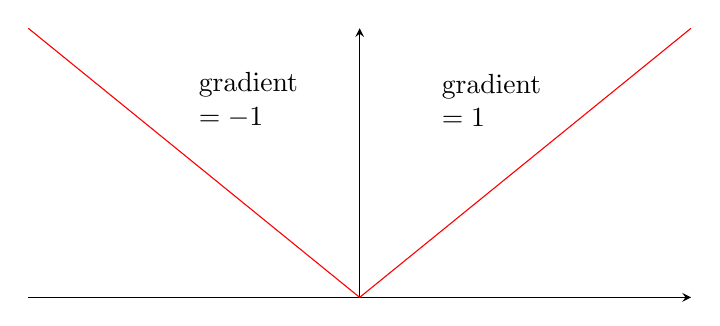
\begin{tikzpicture}
\begin{axis}[
axis lines=middle,
xtick = {0},
xticklabels = {$0$},
ytick = 0,
  width=10cm,height=5cm]
   \addplot[color = red, domain=-0:0.003,smooth]{x};
   \addplot[color = red, domain=-0.003:0,smooth]{-x};
   \node[text width = 1cm] at (axis cs: 0.0011,0.0022) {gradient  $= 1$};
   \node[text width = 1cm] at (axis cs: -0.0011,0.0022) {gradient $= -1$};
 \end{axis}
\end{tikzpicture}
\end{center}




So left and right derivates do exist, they're just not equal. 
\end{example}\vspace*{5pt}

\begin{definition}
Left derivative of $f$ at $a$ is $\lim_{x \to a^-}\frac{f(x) -f(a)}{x-a}$ iff it exists. Right derivative is $\lim_{x \to a^+}\frac{f(x) -f(a)}{x-a}$. 

$\lim_{x \to a^-}g(x)$ exists and equals $\lim_{x \to a^+}g(x) \iff \lim_{x\to a}g(x)$ exists.
\end{definition}

So $f$ is differentiable at $a$ iff the left and right derivatives of $f$ exist at $a$ and are equal. 

Anything else you might guess is also false: e.g. ``if $f$ is differentiable everywhere then is $f'$ continuous?'' No!\vspace*{10pt}

\begin{theorem}[Product Rule] $f,g : \RR \to \RR$ differentiable at $a \in \RR$. Then $fg$ is differentiable at $a$ with $(fg)'(a) = f'(a)g(a) + f(a)g'(a)$
\end{theorem}
\begin{proof}
\[\begin{aligned}
	\frac{f(x)g(x) - f(a)g(a)}{x-a} &= \frac{(f(x)-f(a))g(x) + (g(x) - g(a))f(a)}{x-a} \\ 
	&= g(x) \frac{f(x)-f(a)}{x-a} + f(a)\frac{g(x)-g(a)}{x-a}
\end{aligned}
\]
Taking $\lim_{x\to a} \implies (fg)'(a) = g(a)f'(a) + f(a)g'(a)$ by cty of $g$ and algebra of limits.
\end{proof}
\pagebreak

\begin{corollary}
$f(x) = x^k$ has $f'(x) = kx^{k-1}$	
\end{corollary}
\begin{proof}
Induction!	
\end{proof}

Then $g(x) := 1/f(x)$ is defined in a neighbourhood of $a$, and it is differentiable with $g'(a) = \dfrac{f'(a)}{f^2(a)}$

\begin{proof}
See old question sheet.

 $f$ is continuous at $a \implies \exists \delta > 0$ s.t. $\forall x \in (a-\delta,a+\delta),~|f(x)| > \frac{|f(a)|}{2}$. So $g$ is defined on $(a-\delta,a+\delta)$. 
 
 Working on this and $(a-\delta,a+\delta)\ni x$ we calculate
 
 \[\begin{aligned}\frac{g(x) -g(a)}{x-a} &= \dfrac{1/f(x) -1/f(a)}{x-a}\\
 &= \frac{f(a) - f(x)}{(x-a)f(a)f(x)}\\
 &\to -f'(a)\cdot\frac{1}{f(a)f(a)} \text{ as } x \to a
\end{aligned}\]
\end{proof}


\begin{example}
$E(x) = \sum_{n=0}^\infty \frac{x^n}{n!},~x\iR$	

If we could differentiate term by term we would conclude that

\[E'(x) = \sum_{n=1}^\infty \frac{nx^{n-1}}{n!} = \sum_{k=0}^\infty \frac{x^k}{k!} \quad(k=n-1)\]
So Mestel \emph{guesses} that $E' = E$

\textbf{Claim:} $E'(0) = 1$
\begin{proof}
\[\begin{aligned}\frac{E(x) -E(0)}{x-0} &= \frac{\sum \frac{x^n}{n!}}{x}\\
&= \sum_{n=1}^\infty \frac{x^{n-1}}{n!}\\
&= 1 + \sum_{k=1}^\infty \frac{x^k}{(k+1)!} \quad(k = n+1)
\end{aligned}
\]

Now by the comparison test \[\sum_{k=1}^\infty \frac{x^k}{(k+1)!} \leq \sum_{k=1}^\infty |x^k| = \dfrac{|x|}{1-|x|} \to 0\]

So $\lim_{x\to 0} \dfrac{E(x) - E(0)}{x-0}$ exists and equals $1$. 
\end{proof}

So now we have
\begin{proposition}
$E$ is differentiable everywhere with $E' = E$	
\end{proposition}
\begin{proof}

\[\begin{aligned}
\frac{E(x) - E(a)}{x-a} &= E(a)\cdot \frac{E(x-a)-E(a)}{x-a}\\
 &\to E(a)E'(0) \\
&= E(a)	
\end{aligned}
\]	
\end{proof}
\end{example}\vspace*{15pt}


\subsektion{Rolle's Theorem}\vspace*{5pt}


\begin{theorem}[Rolle's Theorem]\lecturemarker{27}{16 March}
	$f:[a,b] \to \RR$ cts on $[a,b]$, differentiable on $(a,b)$ such that $f(a) = f(b)$. Then $\exists c \in (a,b)$ such that $f'(c) = 0$.
\end{theorem}



\begin{center}
\includegraphics[width = 8cm]{rolle.jpg}
\end{center}


\begin{proof}~
\begin{enumerate}
\item[Case 1.] $f$ is constant on $[a,b]$. Then set $c = \frac{a+b}{2},$ so $f'(c) = \lim_{x\to c}\frac{f(x) - f(c)}{x-c} = 0$.
\item[Case 2.] $f$ takes values $< f(a)$. Then replace $f$ by $-f$ and consider Case 3.
\item[Case 3.] $f$ takes values $> f(a)$. Therefore sup $\{f(x): x \in [a,b]\} > f(a)$ by EVT is realised by some $c \in (a,b)$. Now $f'(c) = \lim_{x\to c} \frac{f(x) - f(c)}{x-c}$. Consider
 \[x > c,~f(x) \leq f(c) \implies \frac{f(x) - f(c)}{x-c} \leq 0 \implies \lim_{x \to c^{+}} \frac{f(x) - f(c)}{x-c} \leq 0\]
 \[x < c,~f(x) \leq f(c) \implies \frac{f(x) - f(c)}{x-c} \geq 0 \implies \lim_{x \to c^{-}} \frac{f(x) - f(c)}{x-c} \geq 0 \] 
 Hence  $\dfrac{f(x) - f(c)}{x-c} = 0$.\qedhere 
\end{enumerate}
	
\end{proof}
\pagebreak

\subsektion{Mean Value Theorem}\vspace*{5pt}


\begin{theorem}[Mean Value Theorem]
If $f:[a,b] \to \RR$ is cts on $[a,b]$ and differentiable on $(a,b)$, then $\exists c \in (a,b)$ such that $f'(c) = \dfrac{f(b) - f(a)}{b-a}$.
\end{theorem}


\begin{center}
\includegraphics[width = 9cm]{mvt1.jpg}
\end{center}
Note: we can write this as $f(b) = f(a) + (b-a)f'(c)$, $c \in (a,b)$. Compare this to Taylor's Theorem - we're taking just the first $2$ terms of.

\emph{Idea of Proof:} Turn MVT into Rolle. 

\begin{center}
\includegraphics[width = 12cm]{mvt2.jpg}
\end{center}

\begin{proof}
Let $g(x) = f(x) - \dfrac{f(b) - f(a)}{b-a}(x-a)$, which is cts on $[a,b]$ and diff'ble on $(a,b)$. $g(a) = f(a) = g(b)$. By Rolle's Theorem applied to $g$
\[\exists c \in (a,b)\text{ such that }g'(c) = 0 \implies g'(c) = f'(c) - \dfrac{f(b) - f(a)}{b-a}.\qedhere\]	
\end{proof}\vspace*{5pt}

\begin{corollary}
If $f'(x) = 0~\forall x \in (a,b)$. Then $f$ is a constant: $f(x) = f(a)~\forall x \in [a,b]$
\end{corollary}
\begin{proof}
Suppose for a contradiction that $\exists d \in[a,b]$ s.t. $f(d) \neq f(a)$. Then by MVT applied to $\left. f\right|_{[a,d]}: [a,d] \to \RR$, $\exists c\in(a,d)$ s.t. $f'(c) = \dfrac{f(d) - f(a)}{d-a} \neq 0,~\cont$	
\end{proof}


\begin{theorem}[Chain Rule]\lecturemarker{28}{19 March} $g: \RR \to \RR$ diff'ble at $a \in \RR$, $f: \RR \to \RR$ diff'ble at $g(a) \in \RR$, then $f \circ g$ diff'ble at $a$ with $(f\circ g)'(a) =f'(g(a))g'(a)$
\end{theorem}

i.e. \[\left.\frac{d}{dx} f(g(x))\right|_{x=a} = \frac{df}{dx} (g(a)) \frac{dg}{dx}(a) = \left.\frac{df}{dy}\right|_{y=g(a)}\frac{dg}{dx}(a) ``=" \frac{df}{dg}\frac{dg}{dx}\]

\emph{Idea of proof:} 
\[\frac{f(g(x))-f(g(a))}{x-a} = \frac{f(g(x)) - f(g(a))}{g(x) -g(a)}\cdot\frac{g(x)-g(a)}{x-a} \to f'(g(a))\cdot g'(a)\]
problem with this is that $g(x) - g(a)$ might be zero

$\left(\dfrac{h(x) - h(a)}{x-a} \text{ is not defined at } x=a \text{, so define it to be } h'(a) \text{ at } x=a \right)$\\

\begin{proof}
Define $F(g) = \begin{cases}
 	\dfrac{f(y)-f(b)}{g-b} & y \neq b\\
 	f'(g) &  y = b 
 \end{cases}~(\ddagger)$
 where $b = g(a)$. \vspace*{5pt}\\$f$ is diff'ble at $b \implies \lim_{y \to b} F(y) \to f'(b) = F(b)$ as $y \to b$. So $F$ is cts at $b = g(a) ~(*)$. 
 
 $g$ is diff'ble at $a \implies$ cts at $a$. 
 
 By $(*) \implies F \circ g$ is cts at $a \implies F(g(x)) \to F(g(a)) = f'(b)$ as $x \to a ~(**)$. 
 
 So now we can follow the rough proof to write 
 \[\frac{f(g(x)) -f(g(a))}{x} = F(g(x))\frac{g(x) - g(a)}{x-a}\]
 

 
 Now take $\lim_{x\to a}$ to get $(f\circ g)'(a)$ exists and equals $f'(b)g'(a)$ by $(**)$ \end{proof}\vspace*{5pt}
 
 Ex: ``Sum Rule" $f, g$ are differentiable at $a\implies f+g$ are differentiable at $a$ with $(f+g)'(a) = f'(a) + g'(a)$. Pre-ex: Algebra of limit for $\lim_{x\to a}$ is on Question Sheet.\\
 
 \emph{Rough:} $f: \RR\to \RR$ is differentiable and bijective, $g = f^{-1}: \RR \to \RR$.
 
  Suppose $g$ is differentiable. Then by the chain rule $f\circ g(y) = y \implies f'(g(y_0))g'(y_0) = 1~\forall y_0 \implies g'(y) = \frac{1}{f'(g(y))}$. 
  
  Suggests that if $f' \neq 0$, then $g$ is differentiable with derivative $\frac{1}{f'\circ g}$\vspace*{5pt}

\begin{theorem}
	If $f:\RR \to \RR$ is differentiable at $a\in \RR$ with $f'(a) \neq 0$ and $f$ is bijective with inverse $g = f^{-1}$, then $g$ is differentiable at $b = f(a)$ with $g'(b) = \dfrac{1}{f'(g(b))} = \dfrac{1}{f'(a)}.$
\end{theorem}
\begin{proof}
\textit{Lemma:} $f'(a) \neq 0 \implies \exists \delta > 0$ such that $f(x) \neq f(a)$ for $x \in (a-\delta,a + \delta)\backslash\{0\}$.  (Proof is left as exercise - use $\lim_{x\to a}$ definition of $f'$ and MVT) \\

 So $\dfrac{g(y)-g(b)}{y-b} = \dfrac{x-a}{f(x) - f(a)} = 1/\dfrac{f(x)-f(a)}{x-a}$ where $x = g(y),~y \neq b$.
 
 As $y \to b$, $g(y) \to g(b) = a$ since $f$ differentiable at $a \implies f$ cts at $a \implies g$ cts at $b \implies x \to a \implies$ RHS $\to \dfrac{1}{f'(a)}$.	
\end{proof}\vspace*{15pt}



\textbf{Felina.} Suppose $f: \RR \to \RR$ satisfies
\begin{itemize}
\item $f(x) + f(y) = f(x+y)~\forall x,y\iR$
\item $f$ is continuous everywhere	
\end{itemize}

\emph{What if $f$?}

Observe $y = 0: f(x) + f(0) = f(x),~\forall x$, so $f(0) = 0$. 

For $y = 1: f(x) + f(1) = f(x+1)$

\[\begin{aligned}\text{Induction } f(x+2) &= f(x) + f(1) + f(1) \\
f(x+3) &= f(x) + 3f(1)\\
&\vdots \\ 
 f(x+n) &= f(x) + nf(1)\\
\implies f(n) &= nf(1) ~(*)\end{aligned}
\]

Similar mucking about should convince you that $f(x) = xf(1)$. We've proved that for $x\iN$ by $(*)$. $f(1)$ is an unknown constant $c$. [Notice $f(x) = cx$ indeed satisfies the given assumptions]

Notice \lecturemarker{29}{20 March} that $(*)$ holds for $n \iZ$ too
\[f(-n) + f(n) = f(n-n) = f(0) = 0\]
\[\implies f(-n) = -f(n) = -nf(1) = -nc,\quad n \iN\]
$(*)$ also holds for $\QQ$
\[\textstyle{\underbrace{\textstyle{f(\frac{n}{m}) + \dots + f(\frac{n}{m})}}_{m \text{ copies}} = f(\frac{n}{m} + \dots + \frac{n}{m}) =f(n) = cn}\]
\[\textstyle{\implies f(\frac{n}{m}) = c\frac{n}{m} \quad \forall \frac{n}{m} \iQ,~n,n\iZ}\]

\textbf{Claim:} $f(x) = cx$ [$c = f(1)$] $\forall x \iQ$

\emph{Idea:} now is if $x \iR$ then $x$ is close to $y \iQ$. $f$ is continuous $\implies f(x)$ is close to $f(y) = cy$, close to $cx$. So $f(x)$ is arbitrarily ($\forall \epsilon!$) close to $cx \implies f(x) = cx$

(or we could use some machinery to say $\forall x \iR$, $\exists (y_n) \to x$, $y_n \iQ$. Then $f$ is continuous $\implies f(y_n) = cy_n \to f(x)$ and $cy_n \to cx$. So uniqueness of limits $\implies f(x) = cx$.) 

\begin{proof}
Fix $x \iR$. Fix $\epsilon >0$. M1F: $\exists y \iQ$ s.t. $|y-x| < \epsilon \implies |cy - cx| < \epsilon/2$
\[\exists \delta >0\text{ s.t. }|x-y| < \delta \implies |f(x) - f(y)| < \epsilon/2\]

and by M1F again $\exists y\iQ$ s.t. $|y-x| < \mathrm{min}\{\delta,\epsilon/2\}$. 

So $|cy-cx|< \epsilon/2$ and $|f(x) - \equalto{f(y)}{cy}| < \epsilon/2 \implies |f(x) - cx| < 2\epsilon/2 = \epsilon$. 

This is true $\forall \epsilon >0 \implies |f(x) -cx| = 0$
\end{proof}

%%%%%%%%%%%%%%%%%%%%%
\vspace*{20pt}


  \begin{center}
  \includegraphics[width = 5cm]{thomas.jpg}
  \vspace*{20pt}
  
  \textsf{\textbf{- End of Analysis I -}}	
  \end{center}
  
  

\end{document}